\chapter {Jets from Binary Protostars}
\label{BinaryJetsChap}
%\minitoc


In this chapter, we investigate potential models that could explain why multiple systems
predominantly show single jets.
During their formation, stars are supposed
to produce energetic outflows and jets.
However, binary jets have only been observed in a very small number of systems.
% Method
We model numerically 3D binary jets for various outflow parameters.
We also model the propagation of jets from a specific source, namely LDN1551 IRS
5,
using recent observations as constraints for simulations with a new MHD code.
We examine their morphology and dynamics, and produce synthetic emission maps.
% Results
We find that the two jets interfere up to the stage where
one of them is almost destroyed or engulfed into the second one.
We are able to reproduce some of the observational features of LDN1551
such as the bending of the secondary jet.
% Orbiting vs interaction
While the effects of orbital motion are negligible over the jets dynamical
timeline,
their interaction has significant impact on their morphology.
% MHD effects
If the jets are not strictly parallel, as in most observed cases, we show that
the magnetic field can help the collimation and refocusing of both of the two
jets.


\section{Introduction}
\subsection{Jets and star formation}
%
%JETS AND OUTFLOWS
%
%Well-collimated jets occur across a broad range of mass scales from young stellar objects to active galactic nuclei.
%In young stellar objects (YSOs), jets and outflows are often optically observed.
%YSO jets are believed to be launched by means of a magnetic field which is anchored or frozen into a circumstellar disk, and pinched and twisted by the disks rotation. 
%Once the pinched-in field reaches a critical angle, fast-rotating gas from the disk may be loaded onto the field lines and thus launched into the parent cloud in an outflow \citep{1982MNRAS.199..883B}.
%Current schools of thought diverge on whether the wind is launched primarily from the inner disk region (disk-wind , \citep{2000prpl.conf..759K} ) or the X-annulus where the young star's magnetosphere interacts with the disk (X-wind, \citep{2000prpl.conf..789S}). 
%However in either case it is believed that the function of the jet or outflow is to brake the rotation of the disk and is thus essential to the star formation process.
%
% Multiple and Binary stars (Statistics)
%

The majority of stars are binaries or part of multiple systems.
During their formation, most stars are thought to produce energetic outflows and jets.
However, binary jets have only been observed in a very small number of systems.


\subsection{Binary Systems}

The formation of binary systems is still poorly understood. 
%
% Bipolar jets and outflows almost never appear binary or multiple
%
It is well established that multiple sources can be the source of HH objects, e.g. T Tau, IRAS 04325-1419, Z Cma, Sz 68, SR 24, S Cr A, AS 353 \citep{1993ApJ...408L..49R}.
A multiple system may produce a single jet or outflow or a set of multiple outflows.
Depending on the binary separation distance, the disk configuration may either be in circumstellar disks or circumbinary disks \citep{2000prpl.conf..841H}.
Few binary jets from binary protostars have been observed despite estimates which show large majorities of binary and multiple star systems among stellar populations \citep{2002ApJ...581..654P,1995ApJ...443..625S,1993AJ....106.2005G,1992ASPC...32...50Z,1991A&A...248..485D}.
In particular, for low mass pre-main sequence stars the binary fraction was estimated to be 60($\pm$17\%) \citep{1993AJ....106.2005G}.
%\citet{1992ASPC...32...50Z} found a frequency of 20\% 
This implies that there should be ``many'' visible binary jets. 
The examples known to the author are compiled in Table \ref{BinaryOutflowTable}.
The frequency of existing binary jets is low compared to the large number of protostellar binary
sources.  


%
%Example of binary jets
%

\begin{table*}
\begin{center}
\caption{Evidence of Binary Jets and Outflows?}
\label{BinaryOutflowTable}
\begin{tabular}{l l l l l}
\hline
\hline
Outflow (Source)  & Cloud & RA (J2000) & Dec (J2000) & Reference \\
\hline
HH154 (LDN1551 IRS 5)        & Tau-Aur   &  04 31 34.20 & +18 08 04.8 & \citet{2005ApJ...L}\\
HH1-2 - HH144     &  Orion & 05 36 22.85 & -06 46 06.6   & \citet{1993ApJ...408L..49R} \\
HH111 - HH121     & Orion &  05 51 46.07 & +02 48 30.6  & \citet{1994AA...289L..19G} \\
BHR71             & N.A.  &  12 01 37    & -65 08 53.5  & \citet{2006AA...454L..79P} \\
L723 (IRAS 19156+1906)  & Cep & 19 17 53.16 & +19 12 16.6 & \citet{2004RMxAC..21..100A} \\
HH288 (IRAS 00342+6347) & Cep& 00 37 11.07 & +64 03 59.8 & \citet{2001AA...375.1018G} \\
HH377 (IRAS 23011+6126) & Cep E  & 23 03  13.9 & +61 42 21  & \citet{1997ApJ...474..749L} \\
IRAS 16293-2422 & $\rho$ Oph E   & 16 32 22.8 & -24 28 33  & \citet{2001ApJ...547..899H} \\
IRAS 20050+2720 & Cyg Rift    & 20 07 06.7 & +27 28 53 &  \citet{1995ApJ...445L..51B}  \\
%Cep A-HW2            & &  & \\
\hline
\end{tabular}
\end{center}
\end{table*}



\subsection{Models for Binary jets}

%
%Example of binary jets
%
In the models of \citet{1997A&A...319..340F,1987ARA&A..25...23S} and \citet{1987IAUS..115..417S} a single circumstellar disk produces a bipolar outflow or jet.
However, observations have shown that multiple or quadrupolar jets may occur.
\citet{1993ApJ...408L..49R} discovered a second flow HH144 from the same source as HH1-2. 
\citet{1994A&A...289L..19G} observed a second flow (HH121) from the same source as the well-known HH111 outflow.
In both cases there are large angles of separation between the two jets.
However observations of apparent double jets can also be explained by other means: \citet{1990ApJ...357..524A} imaged the outflow in L723 and found a distinct multi-polar morphology. They concluded that the lobes of the jets were in fact shell walls of two cavities swept clear by a single bipolar outflow. \citet{1991ApJ...376..615A} discovered a double radio source at the centre of the outflow structure and this led to a reappraisal of the of the double outflow theory \citep{1996ApJ...473L.123A,1997ApJ...489..734G,1998ASPC..132..303A,1998ApJ...504..334H,1999A&A...346..233P,2002ApJ...575..337S,2003RMxAC..15..135E,2004RMxAC..21..100A}.
Other example of multiple molecular outflows include IRAS 16293-2422,  IRAS 20050+2720.

%
%Goals: study space parameter, comparison with observations, potential origin.\\
%

% Introduction
There are several possible explanations for the apparent paucity of binary jets and outflows.
One possible explanation is simply that the number of binary systems has been overestimated \citep{2006ApJ...640L..63L}.
However this still leaves a large number of known binaries without binary jets or outflows.
Another possibility is that the dust extinction from the circumbinary material may block the smaller outflow from view in some cases.
A third possibility is that the two jets - which launched from roughly the same regions - merge into a single jet.
%This seems quite likely.
A detailed model of binary jets presented here will show the effect of their relative sizes and speeds on their interaction.
%Parameter space
If the disks are not coplanar \citep{1994ARA&A..32..465M} it reasonable to assume that binary outflows can have quite large angular separations.
%are interested in jets with two sources independently driving two bipolar outflows.
% Comparison with Observations
The current study is confined to pairs of jets with small angular separations e.g.\ the binary jet from LDN1551 IRS 5.


% Potential origins

%
%Method
%

% Introduction

% Let's model binary jets and show they don't stay binary for long
%want to model binary jets in detail and demonstrate the effects of their relative sizes and speeds on their interaction.
% by launching jet simulations
Numerical simulations of the binary jet model are performed using a specific object, LDN1551 IRS 5 (HH154) as a starting-point for the model.
% and use an observed object LDN1551 IRS 5





\begin{figure}[t]
\begin{center}
   \begin{minipage}[c]{.48\linewidth}
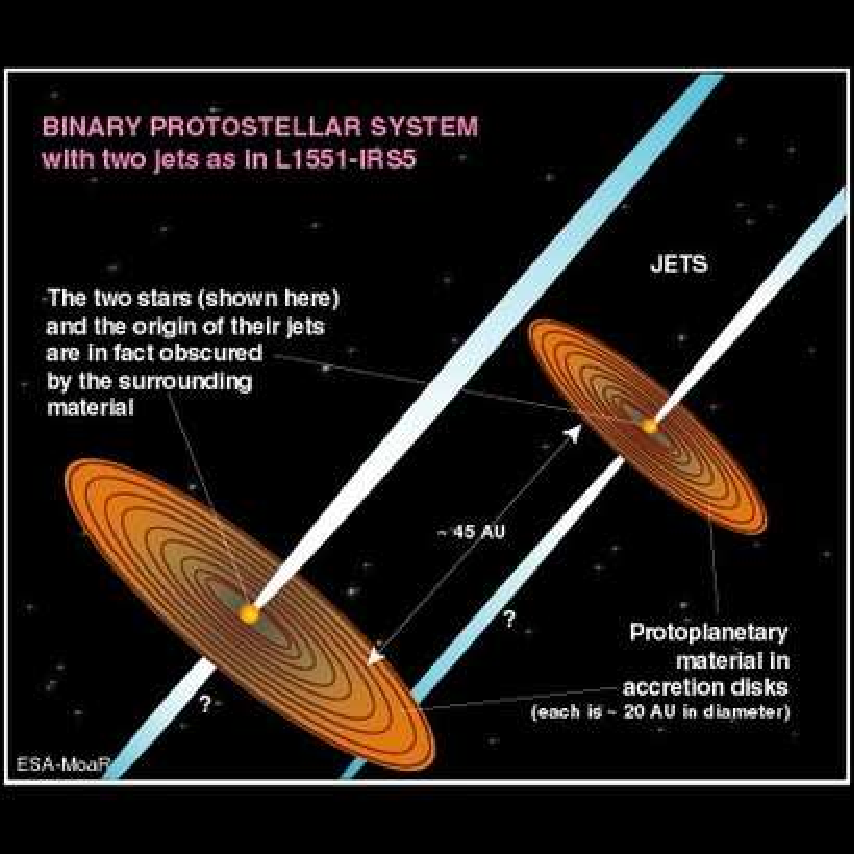
\includegraphics[width=5cm]{schematic_l1551}
   \end{minipage} \hfill
   \begin{minipage}[c]{.48\linewidth}
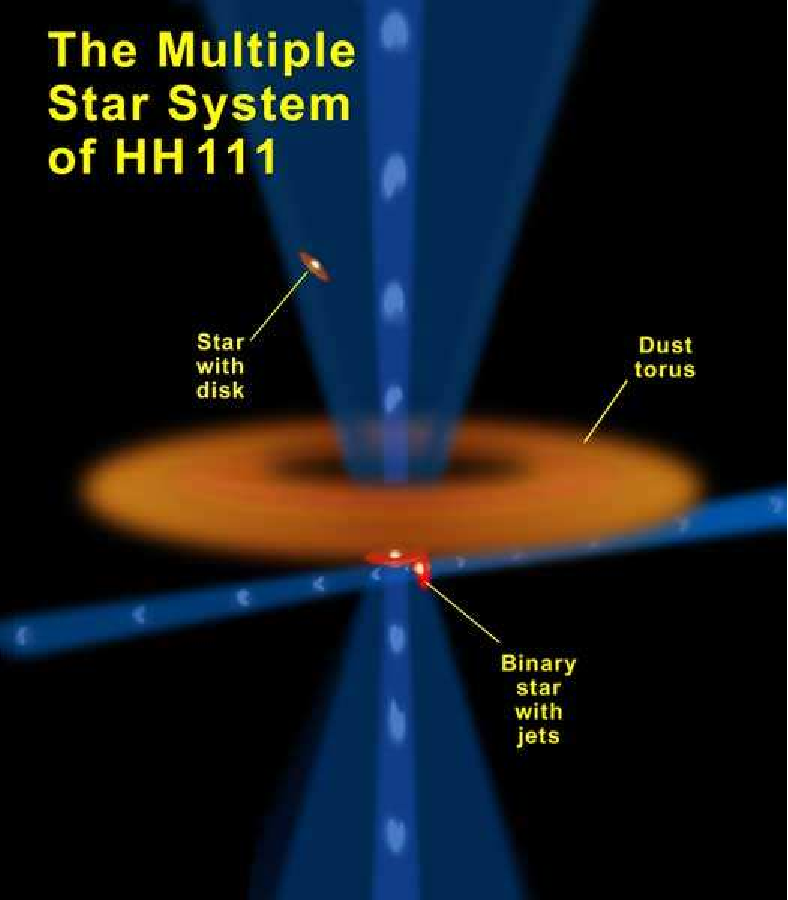
\includegraphics[width=5cm]{schematic_hh111}
   \end{minipage} \hfill

\caption{
Left panel:
Cartoon of LDN1551 IRS 5 jets.
Right panel: 
Cartoon of H111 and HH121 jets.
}
\label{fig:SchemeH111} 
\end{center}
\end{figure}




% Summary of other models 
%Numerical models of optical jets have evolved over the past twenty years, from the original models by \citet{1981ApJ...247...52N} of the \citet{1974MNRAS.169..395B} twin-exhaust model,
%to later models by \citet{1984ApJ...276..560H,1987ApJ...316..323H,1988ApJ...326..323R} which were 1.5D bow shock models which explicitly tried to model observed features, to more complicated geometries and physics including atomic radiative cooling \citet{1998AJ....116.2943R,2000A&A...364..763R,2001A&A...367..959R}.
% Mostly by Raga
A full examination of the interaction of binary jets is impossible to model using axisymmetry.
Therefore a fully three-dimensional binary jet system is modelled using ATLAS, the code introduced in Chapter \ref{NumericalMethod}.


% STRUCTURE OF THE CHAPTER
This chapter is structured as follows: 
in part \ref{Observation_Section} the observations of the source are summarised, 
in part \ref{Simulation_And_Code} the method is described,
in part \ref{Results} the results of the simulation are presented, 
and finally in part \ref{Discussion} the consequences of the model are discussed.

%%%%%%%%%%%%%%%%%%%%%%%%%%%%%%
%%%%%%%%%%%%%%%%%%%%%%%%%%%%%%
\section{Observations of jets from the binary protostar IRS 5}
\label{Observation_Section}
%%%%%%%%%%%%%%%%%%%%%%%%%%%%%%
%%%%%%%%%%%%%%%%%%%%%%%%%%%%%%


\begin{figure}[t]
\centering
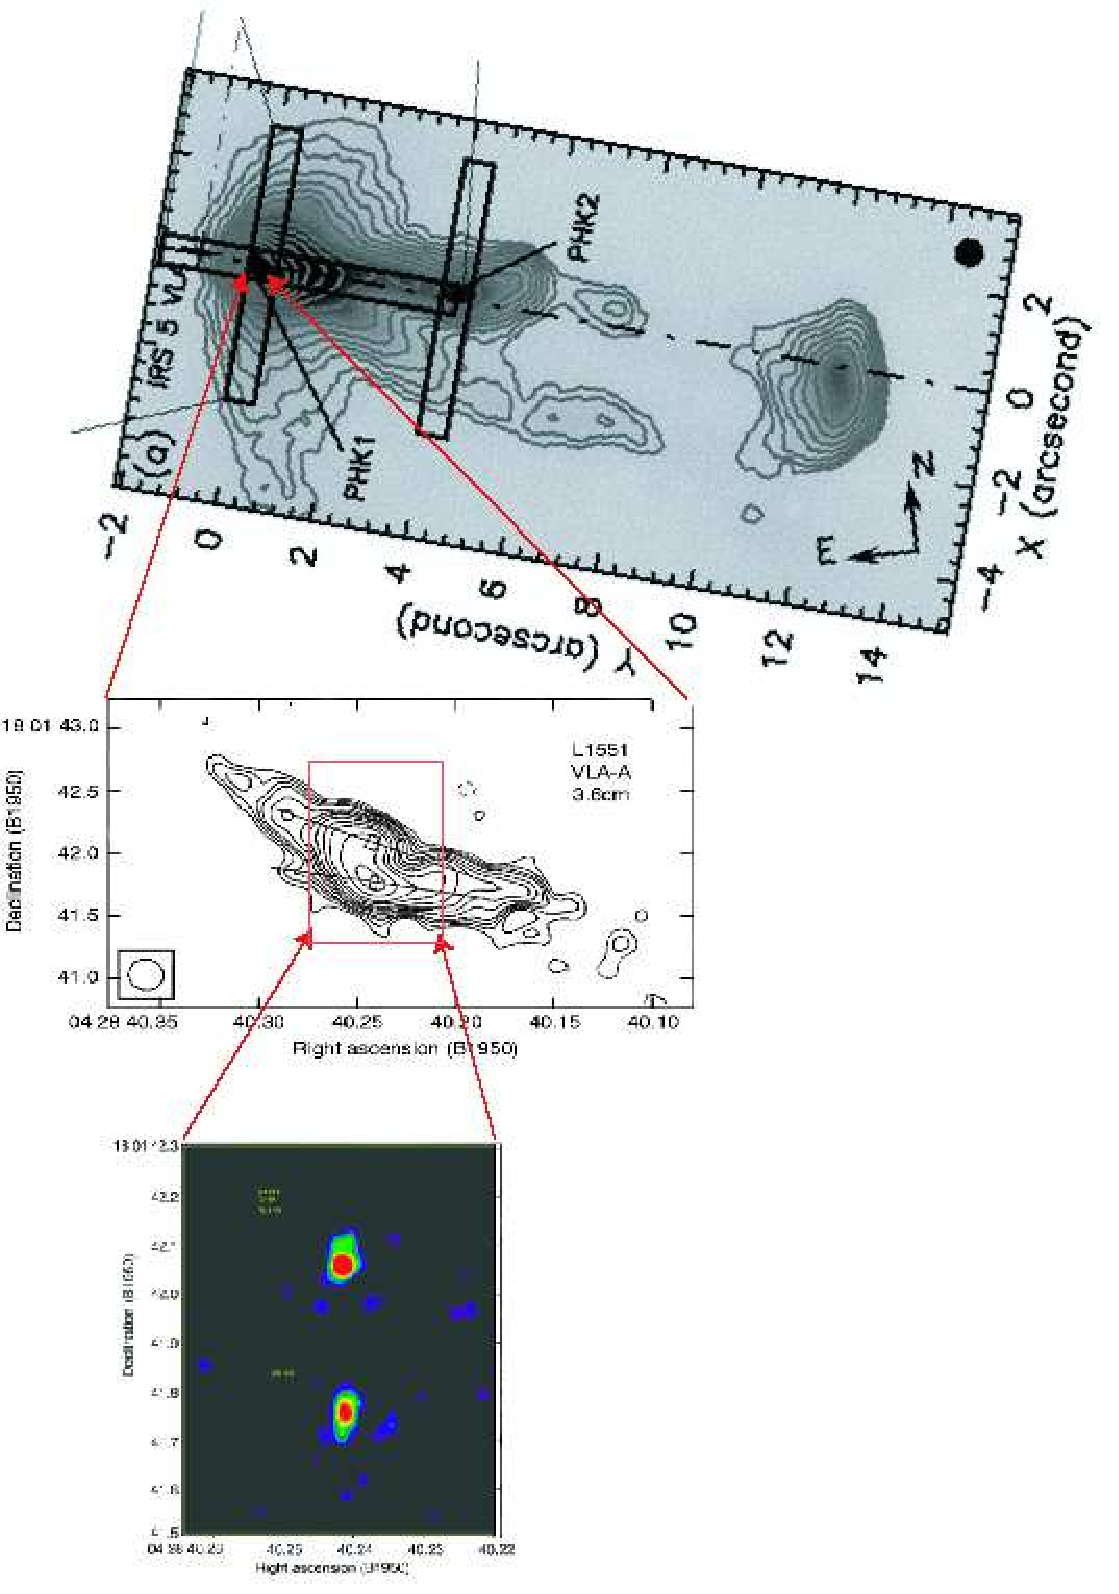
\includegraphics[width=8cm]{FiendishlyGood}
\caption{
Observations of LDN 1551 IRS 5.
The upper panel shows an image of the jet pair in [FeII] from \citet{2002ApJ...570..724P}.
The middle panel is a radio image at $3.6$~cm of the binary jet which shows the blue and red lobes of the binary jets from \citet{1998Natur.395..355R}. The two rectangles at the centre of the image mark the positions of the two disks. The solid lines show the estimated directions of the two disks.
The lower panel is a radio image of the pair disks which drive the binary jets at$7$~mm from \citet{1998Natur.395..355R}.
}
\label{fig:Fiend} 
\end{figure}



\begin{figure}[t]
\centering
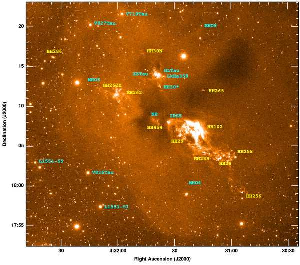
\includegraphics[width=\textwidth]{LDN1551Cloud}
\caption{
Observations of LDN 1551 molecular cloud in [SII] on the Cerro Tololo Telescope, from \citet{2005prpl.conf.8527M}. The infrared source of the binary jets, IRS 5 is located at  RA 04 31 34.20 DEC  +18 08 04.8.
}
\label{fig:Cloud} 
\end{figure}

%LDN1551 IRS 5 has an infrared emission nebulosity \citep{1994ApJS...94..615H}. It is believed that there is a hole perpendicular to the high-density disk and light from the central star escapes through the hole and irradiates the nebulosity.
Using both the Hubble Space Telescope and SUBARU, two optical jets have been observed emanating from LDN1551 IRS5, located 140 parsecs away in the Taurus molecular cloud complex. 
The optical jets extend southwest and disappear
 at  approximately 1400AU from the IRS5, where the large knot of [Fe II] emission is at y=12 arcsec in the upper panel of Figure \ref{fig:Fiend}.
 As for the origin of the two jets, 
 the north and south jets appear to be launched from the south and north disks respectively of the binary system in LDN1551 IRS 5.
 The disks are not seen edge-on, the inclination angle has been estimated at about 45$^{\circ}$.

%A brief overview of the object LDN1551 IRS 5 and its associated jets and outflows is given.
\cite{1976AJ.....81..638S} observed the near-infrared source IRS 5 within the Lynds molecular cloud 1551 (LDN(=Lynd's Dark Nebula) 1551).
\cite{1979AJ.....84..548C} discerned two fast Herbig-Haro objects, HH28 and HH29, near the IRS 5 source.
\cite{1980ApJ...239L..17S} saw for the first time in CO the ``remarkable double-lobed
structure'' in LDN1551, molecular bipolar outflows extending for 0.5 parsecs in opposite directions, with velocities of 15 km~s$^{-1}$.
This was among the first molecular bipolar outflows discovered.
\citet{1985ApJ...289L...5B} identified IRS 5 as a binary source.
\citet{1991ApJ...373L..23M} and \citet{1991ApJ...383..705P} identified a second outflow from the same source.
\citet{1991A&A...252..740M} also observed two independent rows of knots although these were interpreted as edges of a limb-brightened cavity, and were only identified as jets by \citet{1998ApJ...499L..75F} (hereafter FL). 
FL opined that only one jet is currently active.
They also estimated that the jets were almost completely ionised.
FL determined that the angular separation between the jets is approximately $20^{\circ}$. 
\citet{2003ApJ...586L.137R} confirm the jet binarity at radio
wavelengths. 
\citet{1998Natur.395..355R} confirmed that LDN1551 IRS 5 was a binary system and show the first images of the circumbinary disks and the red lobes of the two jets.
Additionally they suggested that there is a circumbinary structure and a large-scale envelope around LDN1551 IRS 5.
\citet{1994ApJ...434L..75L} observed a large circumbinary disk of $\sim 160~\mathrm{AU}$ in diameter.
\citet{2005ApJ...L} provide a value for binary separation of 40 AU. 
An excellent review of the observations until 1997 can be found in \citet{1997IAUS..182...19F}.

% Morphology
\subsection{Morphology}
\citet{2000PASJ...52...81I} observed ``a pair of twisted jets of ionised iron'' from the LDN1551 IRS 5.
They argued that the orbital period of the sources, if equated to the precession of the two jets, is too long to be responsible for the observed twisted morphologies of the jets.
Possible other mechanisms can be magnetic in nature e.g. the Lorentz forces may be strong enough to deflect a jet with a potentially small momentum \citep{1998A&A...334..750F,2000IAUS..200P.112F}. 


% X-ray emission
\subsection{X-ray emission}
Soft X-ray emission with a peak at 1 keV from the region of the head of the north jet was observed by \citet{2002A&A...386..204F}.
\citet{2004A&A...424L...1B} carried out a numerical simulation of the north jet,
using a velocity of $1.4\times10^{3}$ km~s$^{-1}$ for the initial jet velocity
and reproduced the jet head X-ray emission.
%Bally
\citet{2003ApJ...584..843B} performed a higher angular resolution study, finding
a source of X-rays in LDN1551 IRS 5 which they attributed to either fast shocks or
reflected x-rays from IRS 5 scattered out through the outflow cavity.
\citet{2003ApJ...584..843B} put forward several models to explain the X-ray
emission, including the intriguing possibility of a quasi-stationary X-ray
luminous shock maintained by interacting colliding winds between the two protostars.

% Polarimetry
\subsection{Polarimetry}
\citet{1988MNRAS.231P..39S} observed optically a magnetic field perpendicular to
the jet axis, and concluded that it could be explained by a
toroidal field in the cloud around the outflow.
\citet{1997MNRAS.286..895L} also observed this ``peculiar pattern of
alignment''. The physical cause for the polarimetry pattern remains unexplained.

According to \citet{2005ApJ...L} the northern jet is faster with velocity strictly higher than 430 km~s$^{-1}$ whereas the southern jet has velocity at most 65 km~s$^{-1}$.
Recent observational evidence has suggested that the source may have a small
third companion \citep{2005JKAS...38..237L}.


The picture being built up over 25 years of observations is that of a pair of YSOs each with its own associated disk and outflow, the whole structure embedded in a larger circumbinary structure, possibly a disk.

% Table 1 




\begin{table*}
\begin{center}
\begin{tabular}{|l| l|}
\hline
Parameter & Value \\
\hline
N Jet Velocity & 200-430 km~s$^{-1}$   \\
S Jet Velocity & 65 km~s$^{-1}$ \\
Disk Separation & 45 AU \\
Angle Between Jets & $20^{\circ}$ \\
Orbital Period & 255 years \\
Ambient Density & 5000 cm$^{-3}$ \\
Jet Density & 500 cm$^{-3}$ \\
Jet Length & 1400 AU \\
Jet Ion Frac & $\sim$1 \\
\hline
\end{tabular}
\caption{Observed data for LDN1551 IRS 5}
\end{center}
\label{ObservationTable}
\end{table*}




\begin{figure}[t]
\centering
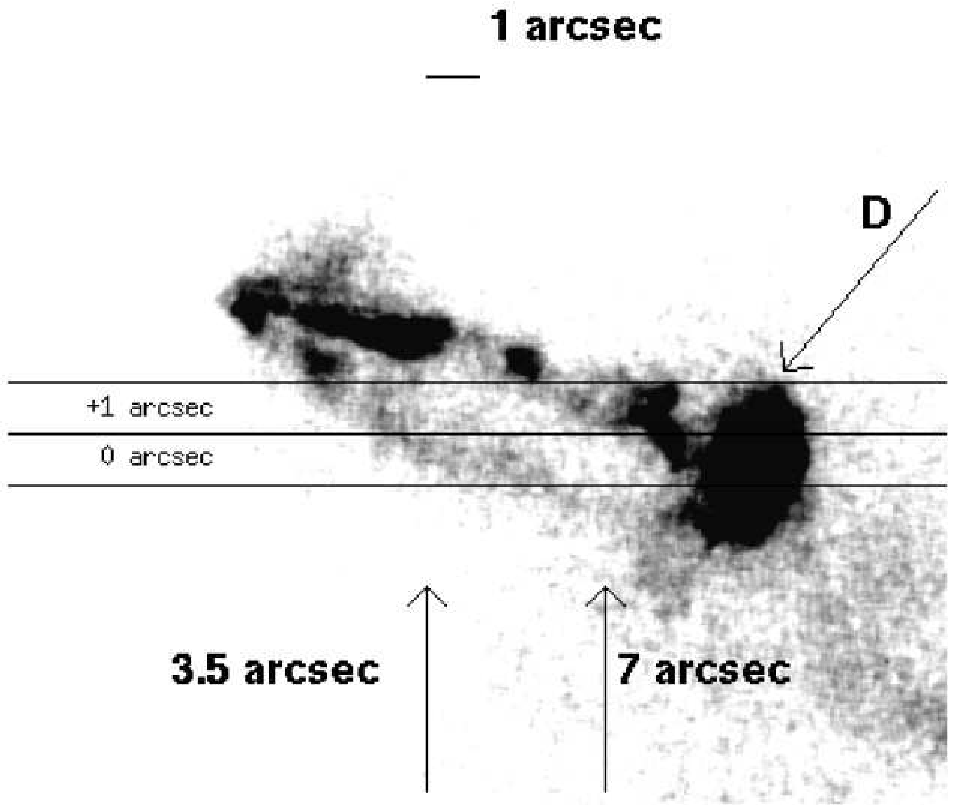
\includegraphics[width=8cm]{l1551_small}
\caption{
\citet{1998ApJ...499L..75F} provide a HST R-band image of the two jets from the
binary protostar LDN1551 IRS 5, located in the constellation Taurus.  (Image courtesy of \citet{1998ApJ...499L..75F}) }
\label{fig:4-1} 
\end{figure}


%%%%%%%%%%%%%%%%%%%%%%%%%%%%%%
%%%%%%%%%%%%%%%%%%%%%%%%%%%%%%
\section{Method}\label{Simulation_And_Code}
%%%%%%%%%%%%%%%%%%%%%%%%%%%%%%
%%%%%%%%%%%%%%%%%%%%%%%%%%%%%%
The main goal is to model binary jets to examine the nature and extent of the interaction between the jets.
Analytical models of single jets have been 
produced by e.g. \citet{1994ApJ...429..781S}, most of those models remain axisymmetric.
However, axisymmetry assumes rotational symmetry in the jet axis and this is not true for binary jets; binary jet propagation and interaction require a full 3D model.
A numerical study becomes necessary, and requires the use of a fully three-dimensional time-dependent model with magnetic field and radiative cooling.
Constraints on current computational capacity require us to make 
certain approximations however so the ideal
magnetohydrodynamic (MHD) approximations are used in order to include the effects of the magnetic field.
The non-ideal physics of optically thin atomic 
radiative cooling losses are included, and the ionisation fraction is tracked in the simulation.
%
%\subsection{System of Equations}
The ideal magnetohydrodynamics (MHD) equations are evolved in time.
The equations are laid out in Section \ref{EquationsofIdealMagnetohydrodynamicsMHD}.
%
%These equations are expressed in terms of the four quantities (two vector and
%two
%scalar) in addition to time t which are conserved in a volume:
%density $\rho$, momentum, $\rho \mathbf u$, magnetic flux density $\mathbf B$ and energy density, $E$.
%
%
%\begin{equation}
%\frac{\partial \rho}{\partial t}+\boldsymbol{\nabla}\cdot(\rho \mathbf u)=0
%\end{equation}
%
%\begin{equation}
%\frac{\partial}{\partial t}\left(
%\rho \mathbf u
%\right)
%+\boldsymbol{\nabla}
%\cdot
%\left[
%\rho \mathbf u \otimes  \mathbf u
%+\left(
%p^*
%\right)
%\mathbf {{\overline {\overline I}}}
%+\mathbf{B} \otimes \mathbf{B}
%\right]
%=0
%\end{equation}
%
%\begin{equation}
%\frac{\partial \mathbf{B} }{\partial t}+
%\boldsymbol{\nabla}
%\cdot
%(
%\mathbf{u} \otimes \mathbf{B}-
%\mathbf{B} \otimes \mathbf{u})
%= 0
%\end{equation}
%
%\begin{equation}
%\frac{\partial E}{\partial t}
%+\boldsymbol{\nabla}
%\cdot
%\left[
%\left( E + p^*\right) \mathbf{u}
%- (\mathbf{u}\cdot\mathbf{B})\mathbf{B}
%\right] + L_{cooling} = 0
%\end{equation}
%
%where $E$ is the total energy, kinetic, internal and magnetic
%\begin{equation} 
%E =
%\frac{1}{2}\rho |\mathbf{u}|^2 + 
%\frac{p}{\gamma-1}+
%\frac{1}{2} |\mathbf{B}|^2
%\end{equation}
%and $p^*$ is the thermal and magnetic pressure:
%\begin{equation} 
%p^* = p + \frac{1}{2}|\mathbf{B}|^2
%\end{equation}
%
%$L_{cooling}$ represents the losses due to optically thin radiative cooling.
%The units are chosen so that $\mathbf B$ absorbs a factor of $1/\sqrt {4 \pi}$.
%The adiabatic index is $\gamma = 5/3$ for a monatomic gas throughout the simulations.
%The equation of state is the ideal gas equation (p=nkT).
%
%\subsection{Microphysics}
%
%Protostellar jets are strongly cooled by optically thin radiative emission.
%It it this emission which render the objects visible.
%Modelling electron transitions directly is neither feasible nor desirable in the
%fluid approximation.
%\citet{1997ApJS..109..517R} identify three main approaches to the inclusion of radiative effects:
%\begin{enumerate}
%\item Assume equilibrium \citep{1987ApJ...323..193R}
%\item Non-equilibrium fully ionised \citep{1990ApJ...360..370B}
%\item Non-equilibrium explicitly computed ionisation fraction \citep{1995MNRAS.272..785F}
%\end{enumerate}
%% use Falle and Raga 
%The third approach is used.
%The microphysics of energy lost due to radiative cooling is represented using a
%cooling function adapted from \citet{1993ApJS...88..253S} and depicted in Figure
%\ref{fig:4-33}, which represents on a macroscopic scale the rate of energy loss at this temperature range for a sample (solar) set of abundances.
%\citet{1993ApJS...88..253S} include the effects of electron collisional ionisation, radiative and dielectronic recombination and line radiation within their cooling function.
%
%\begin{figure}[t]
%\centering
%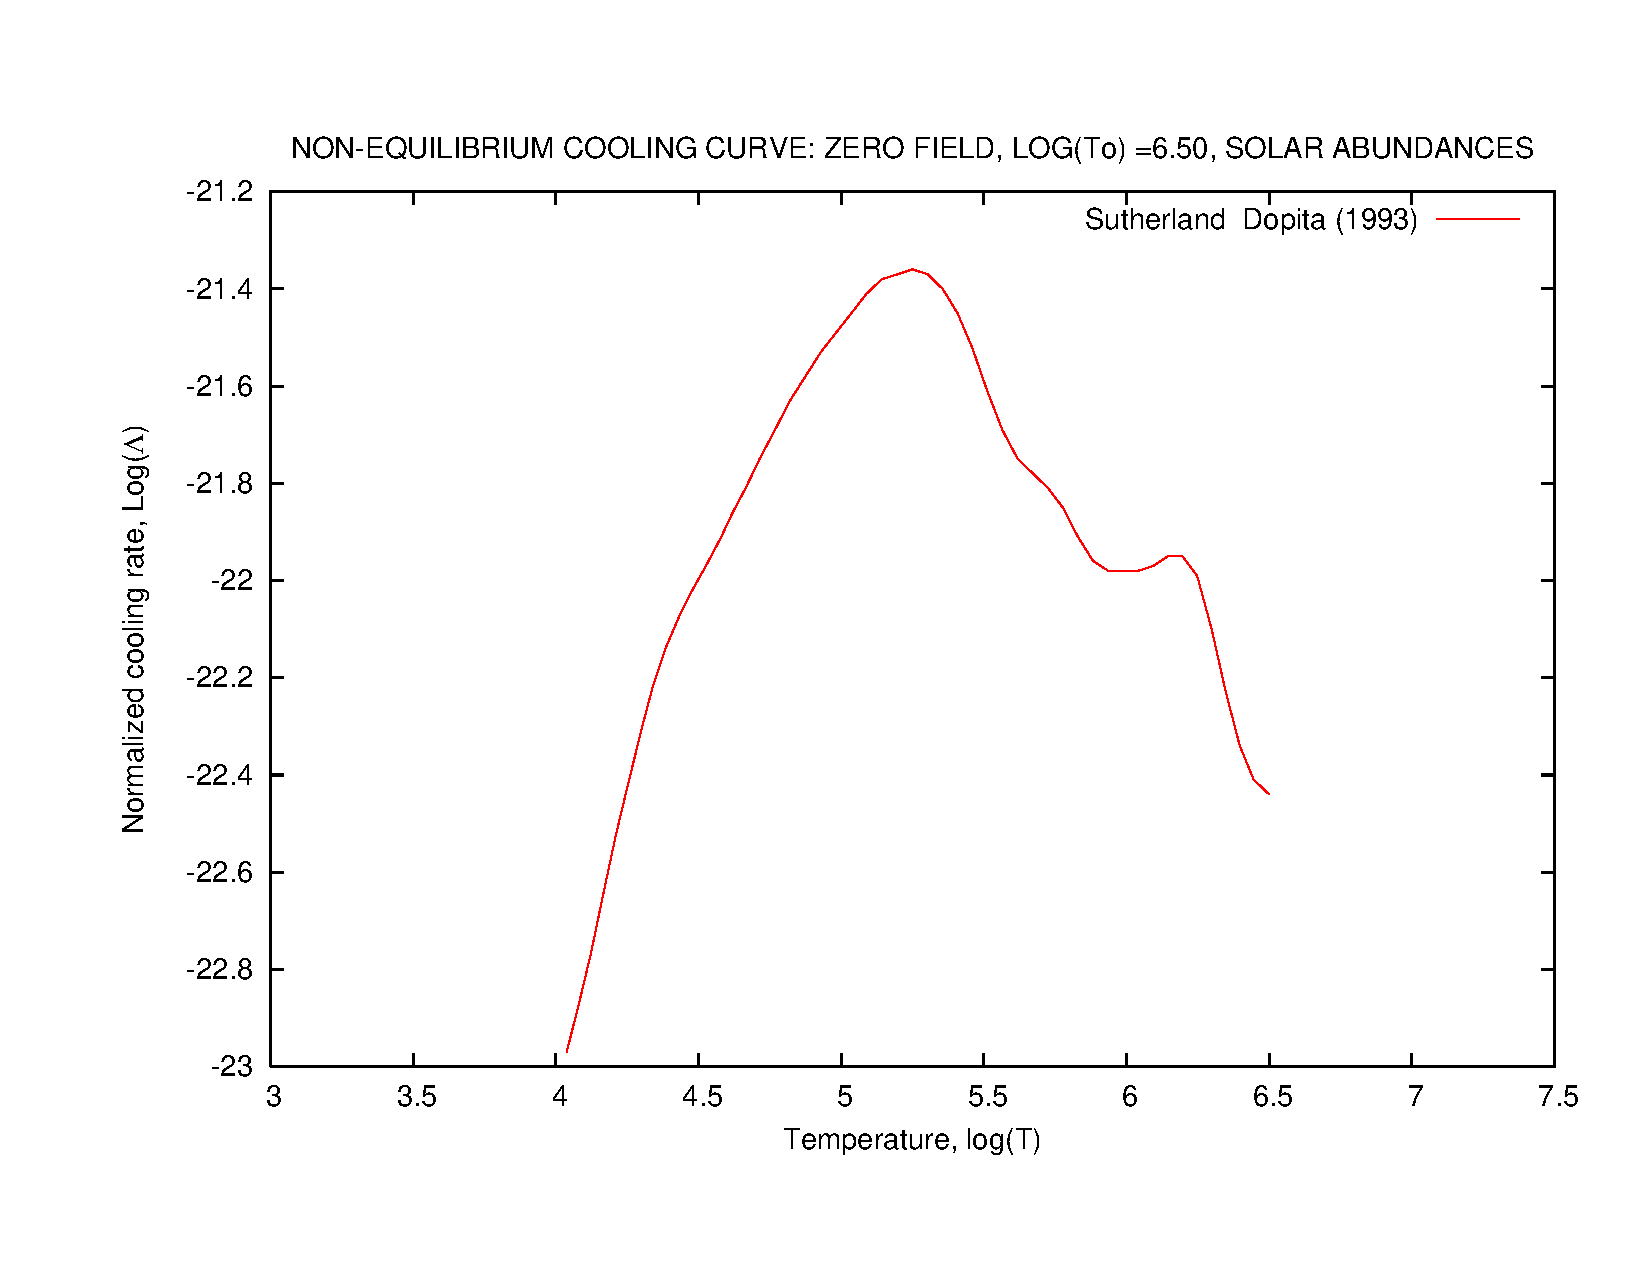
\includegraphics[angle=270,width=8cm]{sutherland}
%%GNUPLOT: LaTeX picture with Postscript
\begin{picture}(0,0)%
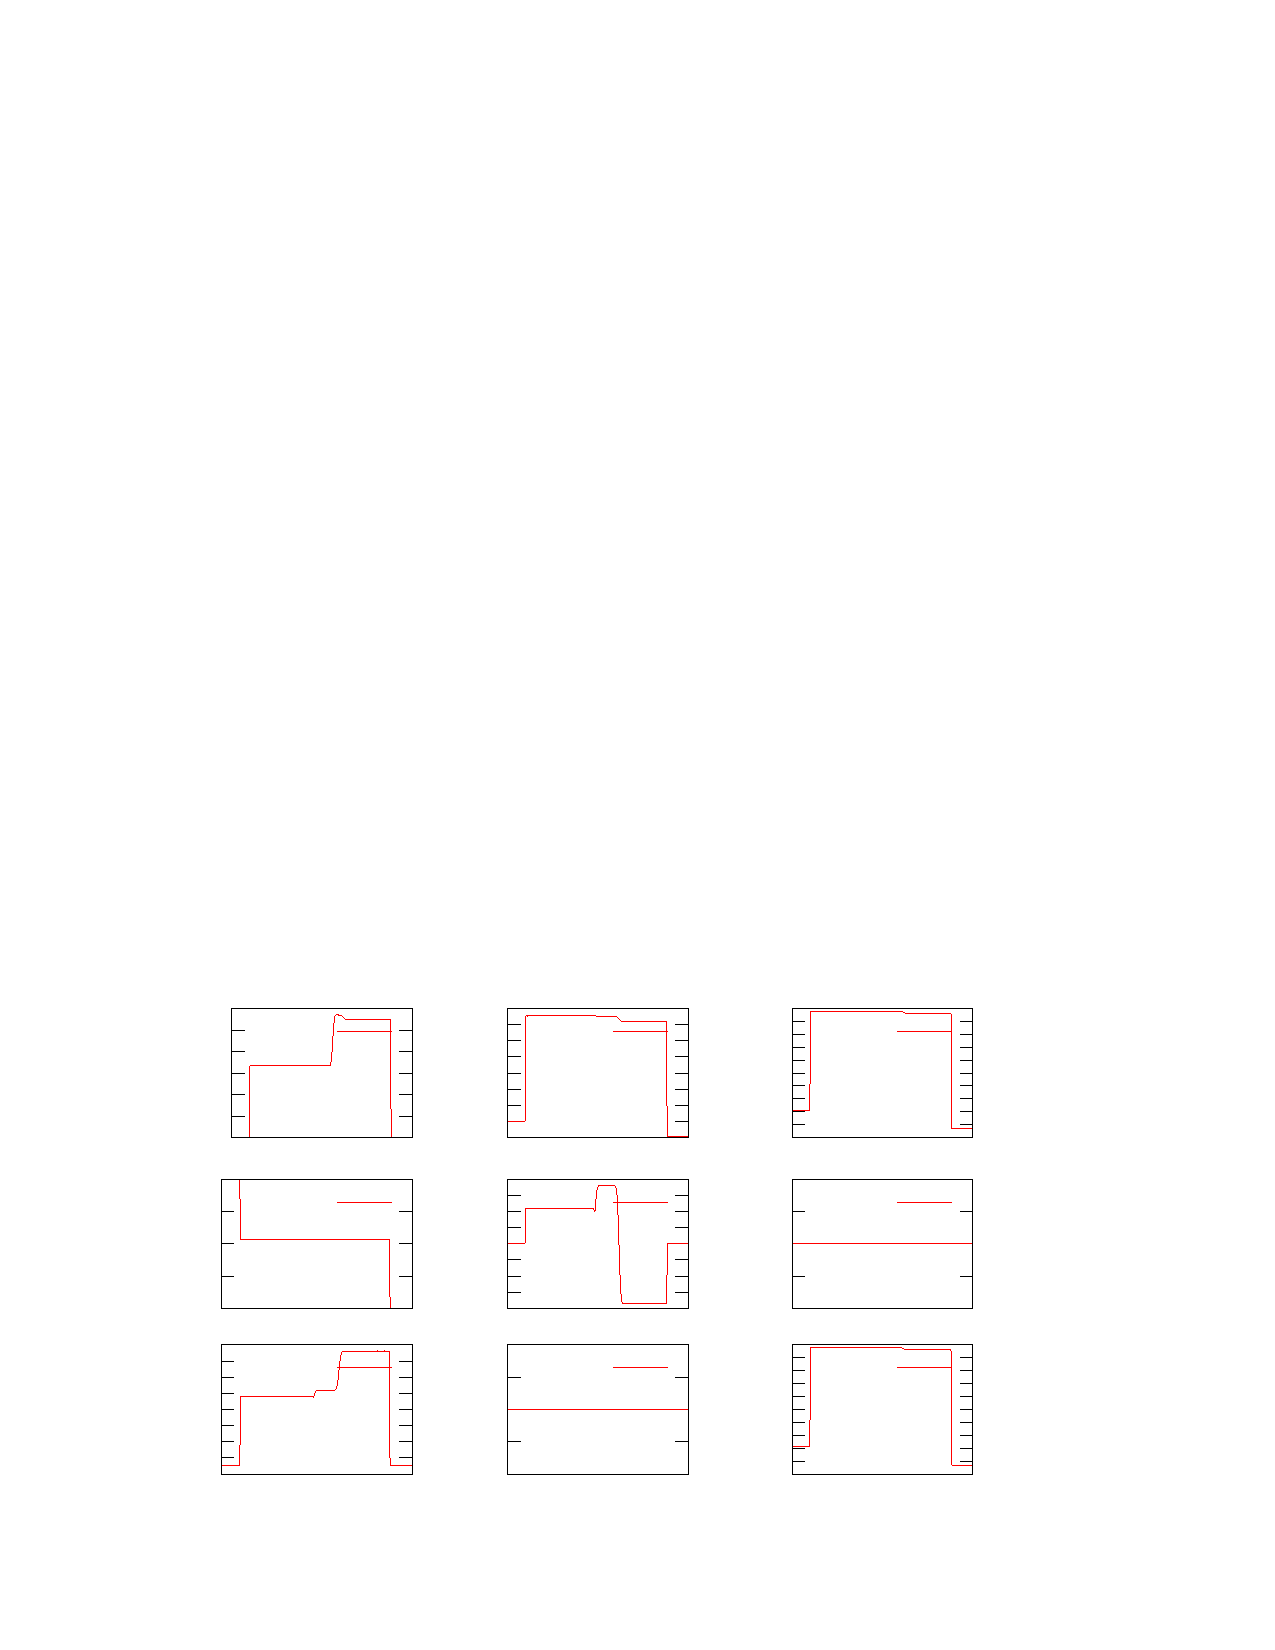
\includegraphics{epslatex/rj1a}%
\end{picture}%
\begingroup
\setlength{\unitlength}{0.0200bp}%
\begin{picture}(20699,12419)(0,0)%
\put(1707,8697){\makebox(0,0)[r]{\strut{} 1}}%
\put(1707,9214){\makebox(0,0)[r]{\strut{} 1.5}}%
\put(1707,9730){\makebox(0,0)[r]{\strut{} 2}}%
\put(1707,10247){\makebox(0,0)[r]{\strut{} 2.5}}%
\put(1707,10763){\makebox(0,0)[r]{\strut{} 3}}%
\put(1707,11280){\makebox(0,0)[r]{\strut{} 3.5}}%
\put(1707,11796){\makebox(0,0)[r]{\strut{} 4}}%
\put(4238,11246){\makebox(0,0)[r]{\strut{}$\rho$}}%
\put(8331,8697){\makebox(0,0)[r]{\strut{} 0}}%
\put(8331,9084){\makebox(0,0)[r]{\strut{} 20}}%
\put(8331,9472){\makebox(0,0)[r]{\strut{} 40}}%
\put(8331,9859){\makebox(0,0)[r]{\strut{} 60}}%
\put(8331,10246){\makebox(0,0)[r]{\strut{} 80}}%
\put(8331,10634){\makebox(0,0)[r]{\strut{} 100}}%
\put(8331,11021){\makebox(0,0)[r]{\strut{} 120}}%
\put(8331,11409){\makebox(0,0)[r]{\strut{} 140}}%
\put(8331,11796){\makebox(0,0)[r]{\strut{} 160}}%
\put(10862,11246){\makebox(0,0)[r]{\strut{}$p_g$}}%
\put(15162,8697){\makebox(0,0)[r]{\strut{} 40}}%
\put(15162,9007){\makebox(0,0)[r]{\strut{} 60}}%
\put(15162,9317){\makebox(0,0)[r]{\strut{} 80}}%
\put(15162,9627){\makebox(0,0)[r]{\strut{} 100}}%
\put(15162,9937){\makebox(0,0)[r]{\strut{} 120}}%
\put(15162,10246){\makebox(0,0)[r]{\strut{} 140}}%
\put(15162,10556){\makebox(0,0)[r]{\strut{} 160}}%
\put(15162,10866){\makebox(0,0)[r]{\strut{} 180}}%
\put(15162,11176){\makebox(0,0)[r]{\strut{} 200}}%
\put(15162,11486){\makebox(0,0)[r]{\strut{} 220}}%
\put(15162,11796){\makebox(0,0)[r]{\strut{} 240}}%
\put(17693,11246){\makebox(0,0)[r]{\strut{}E}}%
\put(1457,4599){\makebox(0,0)[r]{\strut{}-10}}%
\put(1457,5374){\makebox(0,0)[r]{\strut{}-5}}%
\put(1457,6148){\makebox(0,0)[r]{\strut{} 0}}%
\put(1457,6923){\makebox(0,0)[r]{\strut{} 5}}%
\put(1457,7697){\makebox(0,0)[r]{\strut{} 10}}%
\put(4238,7147){\makebox(0,0)[r]{\strut{}V$_x$}}%
\put(8331,4599){\makebox(0,0)[r]{\strut{}-0.4}}%
\put(8331,4986){\makebox(0,0)[r]{\strut{}-0.3}}%
\put(8331,5373){\makebox(0,0)[r]{\strut{}-0.2}}%
\put(8331,5761){\makebox(0,0)[r]{\strut{}-0.1}}%
\put(8331,6148){\makebox(0,0)[r]{\strut{} 0}}%
\put(8331,6535){\makebox(0,0)[r]{\strut{} 0.1}}%
\put(8331,6923){\makebox(0,0)[r]{\strut{} 0.2}}%
\put(8331,7310){\makebox(0,0)[r]{\strut{} 0.3}}%
\put(8331,7697){\makebox(0,0)[r]{\strut{} 0.4}}%
\put(10862,7147){\makebox(0,0)[r]{\strut{}V$_y$}}%
\put(15162,4599){\makebox(0,0)[r]{\strut{}-1}}%
\put(15162,5374){\makebox(0,0)[r]{\strut{}-0.5}}%
\put(15162,6148){\makebox(0,0)[r]{\strut{} 0}}%
\put(15162,6923){\makebox(0,0)[r]{\strut{} 0.5}}%
\put(15162,7697){\makebox(0,0)[r]{\strut{} 1}}%
\put(17693,7147){\makebox(0,0)[r]{\strut{}V$_z$}}%
\put(1457,624){\makebox(0,0)[r]{\strut{} 4}}%
\put(1457,1011){\makebox(0,0)[r]{\strut{} 6}}%
\put(1457,1399){\makebox(0,0)[r]{\strut{} 8}}%
\put(1457,1786){\makebox(0,0)[r]{\strut{} 10}}%
\put(1457,2174){\makebox(0,0)[r]{\strut{} 12}}%
\put(1457,2561){\makebox(0,0)[r]{\strut{} 14}}%
\put(1457,2948){\makebox(0,0)[r]{\strut{} 16}}%
\put(1457,3336){\makebox(0,0)[r]{\strut{} 18}}%
\put(1457,3723){\makebox(0,0)[r]{\strut{} 20}}%
\put(4238,3173){\makebox(0,0)[r]{\strut{}B$_y$}}%
\put(8331,624){\makebox(0,0)[r]{\strut{}-1}}%
\put(8331,1399){\makebox(0,0)[r]{\strut{}-0.5}}%
\put(8331,2174){\makebox(0,0)[r]{\strut{} 0}}%
\put(8331,2948){\makebox(0,0)[r]{\strut{} 0.5}}%
\put(8331,3723){\makebox(0,0)[r]{\strut{} 1}}%
\put(10862,3173){\makebox(0,0)[r]{\strut{}B$_z$}}%
\put(15162,624){\makebox(0,0)[r]{\strut{} 40}}%
\put(15162,934){\makebox(0,0)[r]{\strut{} 60}}%
\put(15162,1244){\makebox(0,0)[r]{\strut{} 80}}%
\put(15162,1554){\makebox(0,0)[r]{\strut{} 100}}%
\put(15162,1864){\makebox(0,0)[r]{\strut{} 120}}%
\put(15162,2173){\makebox(0,0)[r]{\strut{} 140}}%
\put(15162,2483){\makebox(0,0)[r]{\strut{} 160}}%
\put(15162,2793){\makebox(0,0)[r]{\strut{} 180}}%
\put(15162,3103){\makebox(0,0)[r]{\strut{} 200}}%
\put(15162,3413){\makebox(0,0)[r]{\strut{} 220}}%
\put(15162,3723){\makebox(0,0)[r]{\strut{} 240}}%
\put(17693,3173){\makebox(0,0)[r]{\strut{}$\phi$}}%
\end{picture}%
\endgroup
\endinput

%\caption{
%Log normalised radiative cooling loss plotted against log temperature \citep{1993ApJS...88..253S}.
%}
%\label{fig:4-33}\end{figure}
%
%
%\begin{figure}[t]
%\centering
%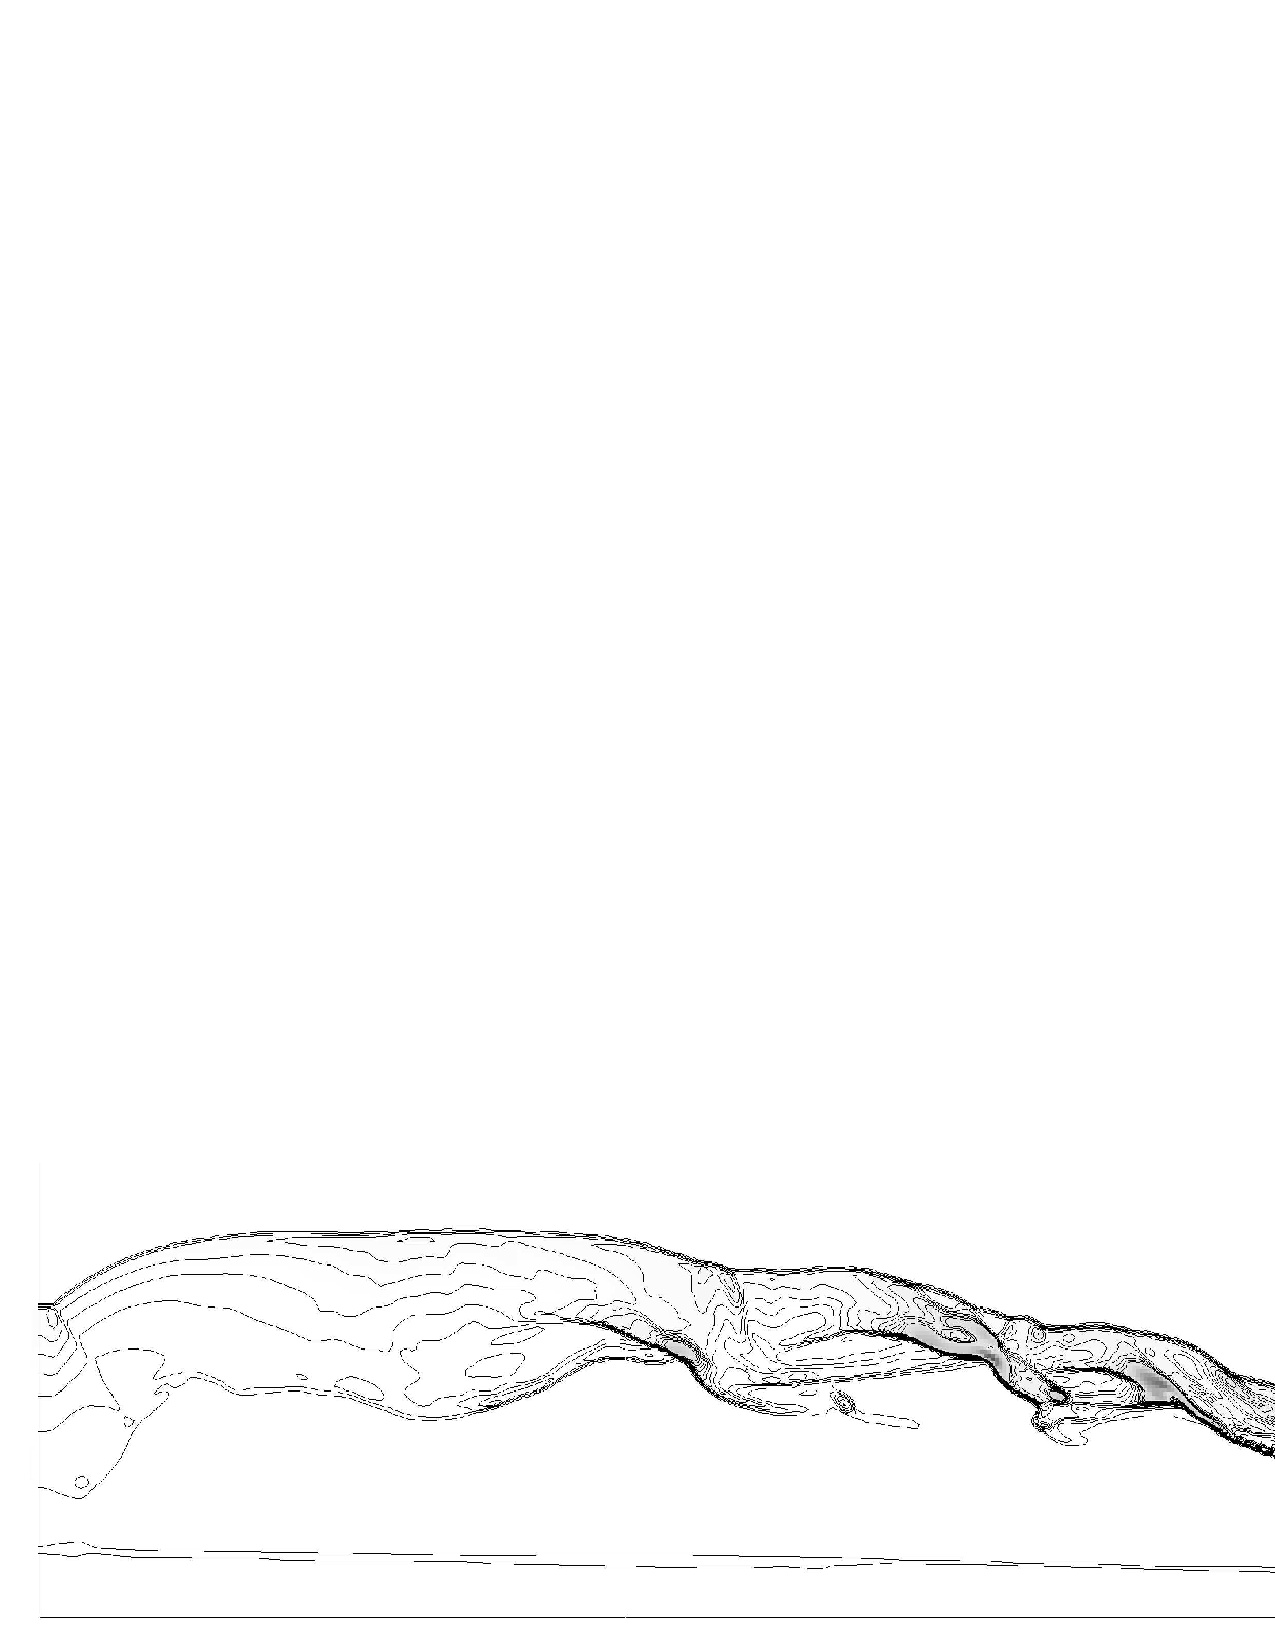
\includegraphics[width=8cm]{cooling}
%\caption{
%Density contours for 300~km~s$^{-1}$ purely hydrodynamical jet with atomic radiative cooling at $t=317$ years.
%The adiabatic atomic jet has a bow shock which has been broken up by cooling - which causes a loss of the pressure which supports the bow shape.
%}
%\label{fig:4-2} 
%\end{figure}
%
%\subsection{The numerical code}
%
% Validation and verification tests including but not limited to the
%Orszag-Tang MHD vortex, the Brio-Wu and Ryu-Jones suite of shock tube tests and 2D and 3D blast wave tests have been run against the code to build confidence in its ability to form correct solutions. 
%ATLAS uses the PARAMESH \citep{par:00} hierarchical block-structured adaptive mesh refinement for high effective resolution in areas of physical interest.  
%The solenoidal constraint ($\boldsymbol{\nabla}\cdot \mathbf{B} =0$) is preserved using a staggered mesh algorithm based on the \citet{307327} field transport method. 
%ATLAS uses a Piecewise Parabolic scheme \citep{1984jcp_colella_woodward} to reconstruct the values at cell interfaces and the Roe-Balsara approximate MHD Riemann solver \citep{Roe81:_approx,Roe:1996:NEM} to explicitly compute the cell interfaces fluxes.
%The multidimensional correction used to compute the transverse fluxes is the Corner Transport Upwind scheme of \citet{Colella90:_multida} as modified by \citet{Saltzman94:_an_uns}.
%
Simulations were carried out using ATLAS (see Chapter \ref{NumericalMethod} for a description) on a 64 node ``Beowulf'' cluster.


\subsection{Initial and boundary conditions}
A distance of 140 parsecs to the jets is assumed. 
%Observed 
Values for the density, temperature and velocities are based on the observations discussed above.
A sinusoidally varying injection velocity
\citep{1990ApJ...364..601R} is assumed, with an amplitude of
$\pm$30\% in the velocity and a period of 8 years for each jet. 
The ambient medium is modelled
with a uniform density ($\rho_a=5 \times 10^{3}$~cm$^{-3}$) and temperature
($10^2 K$) and the jets are modelled with density $\rho_{jet}=0.1\rho_a$,
temperature 10$^4$K and velocities of 65 and 300~km~s$^{-1}$ respectively
\citep{2005ApJ...L}. A compromise figure of 300~km~s$^{-1}$ is chosen between the
estimates of \citet{2005ApJ...L} and \citet{2000AJ....119.1872H}. 
The separation distance between the jets is $2 \times 10^{15}$~cm.
The launching of the two jets is also staggered, the faster northern jet is launched 150 years after the slower southern jet. (The launch times are predicted from the dynamical ages of the jets.)
The velocity radial profile is a positive cosine - with its maximum, v$_{jet}$ at r=0 in the jet centre, dropping to zero at r$_{jet}$. This profile is chose based on the observations of  \citet{2000ApJ...537L..49B}, where the highest velocities are thought to be located in the centre of the jet.
The sheared profile is also consistent with the core/sheath morphology seen in \citet{2002ApJ...576..204H} and \citet{2000ApJ...540..342F}.


% Table 2 
\begin{table}
\begin{center}
\begin{tabular}{l r}
Domain & $-240 $AU$<y,z<240$ AU \\
 & 0$<x<$1440 AU \\
Coarsest grid & $\Delta x=\Delta y=\Delta z=268$ AU \\
Finest grid & $\Delta x=\Delta y=\Delta z=4$ AU \\
Refinement & 5 levels \\
N Jet velocity & $v_{jet}=300~$km~s$^{-1}$ \\
S Jet velocity & $v_{jet}=65~$km~s$^{-1}$ \\
Jet density & $\rho_{jet}=500~$cm$^{-3}$ \\
Ambient density & $\rho_a=5000~$cm$^{-3}$ \\
Jet Temperature & $T_{jet}=10^4 K$ \\
Jet Radii & $r_{jet}=4\times10^{14} $ cm \\
Jet Separation & $s_{jet}=2\times10^{15} $ cm \\
N Jet Mach Number & M=60 \\
S Jet Mach Number & M=12 \\
Ambient Temp & $T_a=100 K$ \\
\end{tabular}
\caption{Initial conditions}
\end{center}
\end{table}

The boundary conditions are inflow for $r<r_{jet}$, reflecting for $r>r_{jet}$ along the inner x-boundary (x=0) and outflow along all other boundaries. 
%%%%%%%%%%%%%%%%%%%%%%%%%%%%%%
%%%%%%%%%%%%%%%%%%%%%%%%%%%%%%
\section{Results}\label{Results}
%%%%%%%%%%%%%%%%%%%%%%%%%%%%%%
%%%%%%%%%%%%%%%%%%%%%%%%%%%%%%

Results from fully 3D HD and MHD simulations of the jets from the
binary protostar LDN1551 IRS 5 are presented, which approximate the physical conditions
producing the morphology in the emission.

\subsection{Case I: HD}
For the hydrodynamic case it is assumed the jets are initially
parallel, which is how the LDN1551 jets appear. The jet
interaction and its effect on the propagation of both jets is modelled.

\begin{figure}[t]
\centering
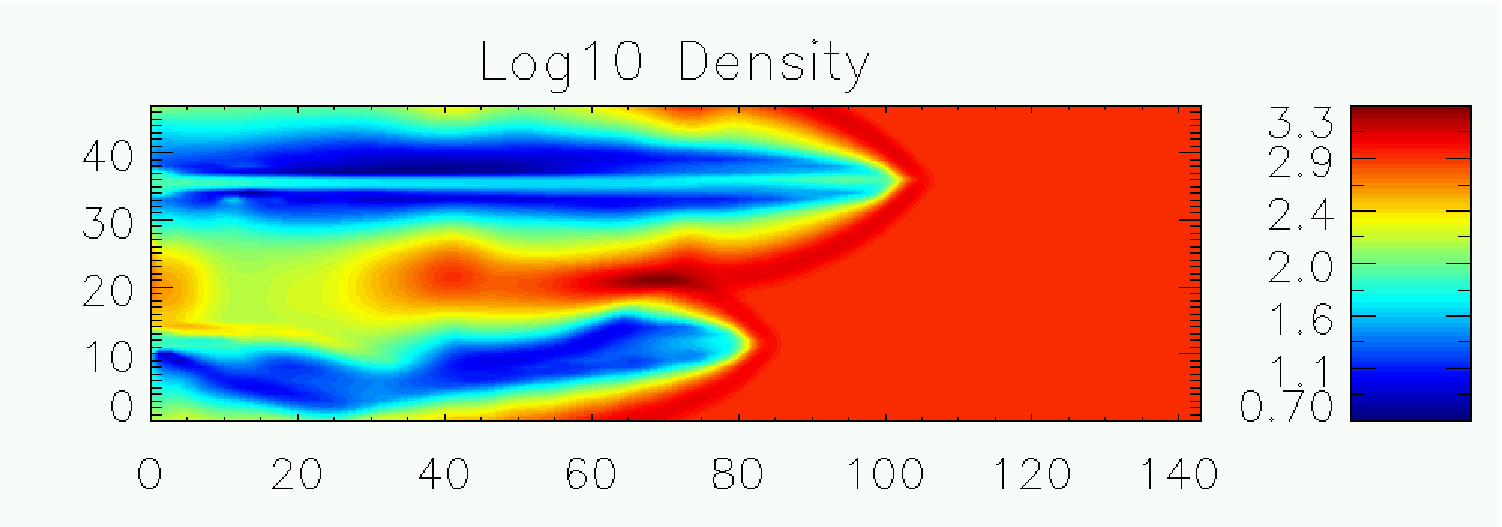
\includegraphics[width=8cm]{3d_slice}
\caption{ 
The bent morphology of the southern (lower) jet is visible in this midplane
colour density map of 3-D binary jet simulation at $t=245~\mathrm{years}$.
The scale of the grid is $1500 \mathrm{AU}$ by $400 \mathrm{AU}$.
}
\label{fig:4-5} 
\end{figure}

The density slice from the 3D HD simulation (see Figure  \ref{fig:4-5}) clearly shows that the slow, secondary jet appears to bend close to the inlet.
Such a bend or kink is also observed in the slow, southern jet of LDN1551 IRS 5 about 4$^{\prime\prime}$ (560 AU at a distance of 140 pc
from the source \citep{2000PASJ...52...81I}).
% There is a kink in the observation
% And in the simulations 
In the simulation shown in Figure \ref{fig:4-5} a kink in the slow southern jet
is also visible - both in the density midplane cut shown in Figure \ref{fig:4-5}
and in the derived emission maps shown in \ref{fig:4-21}. This is caused by 
the bow shock of the fast jet interacting with the beam of the slow jet.
The northern jet has a Mach number $\sim 3$ times higher
than the slow southern jet and simply pushes it out of the way.  This
reproduces the observed kink at 4$^{\prime\prime}$  - without the need for magnetic
fields.  There is no noticeable reaction by the fast jet - possibly
indicating that the estimated velocity is too high.
By using simple hydrodynamical models
the bent morphology of the LDN1551 IRS 5 outflow is reproduced using jet interaction.

\subsection{Case II: MHD}
\label{sec:BinJetMHD}

In the second case, the jet behaviour closer to the source is explained.
The parallel approximation is removed and an angular separation estimated 
at 20$^\circ$ is used. To redirect the two jets would require either a density contrast 
e.g. the wall of a conveniently shaped cavity or a magnetic hoop stress
\citep{2003ApJ...584..843B}.

The magnetic field configuration based on the observations 
of \citet{1988MNRAS.231P..39S} is used. \citet{1988MNRAS.231P..39S} observed 
optically a magnetic field perpendicular to the jet axis, and 
concluded that it could be explained by a toroidal field. The toroidal field may be
produced by the circumbinary material twisting the frozen-in local magnetic field lines. 

In the ambient medium a toroidal field with a maximum value of B=10 $\mu$G is initialised. The magnetic
vector potential ${\mathbf A}$, where ${\mathbf B = \boldsymbol{\nabla}} \times {\mathbf A}$,
had the analytical form A$_x \propto \cos 2 \pi  y + \cos 2 \pi  z.$
This is consistent with the observations \citep{1988MNRAS.231P..39S}.
%This is an approximation to the real field which would be helical according to the disk-twisting theory.

\begin{figure}[t]
\centering
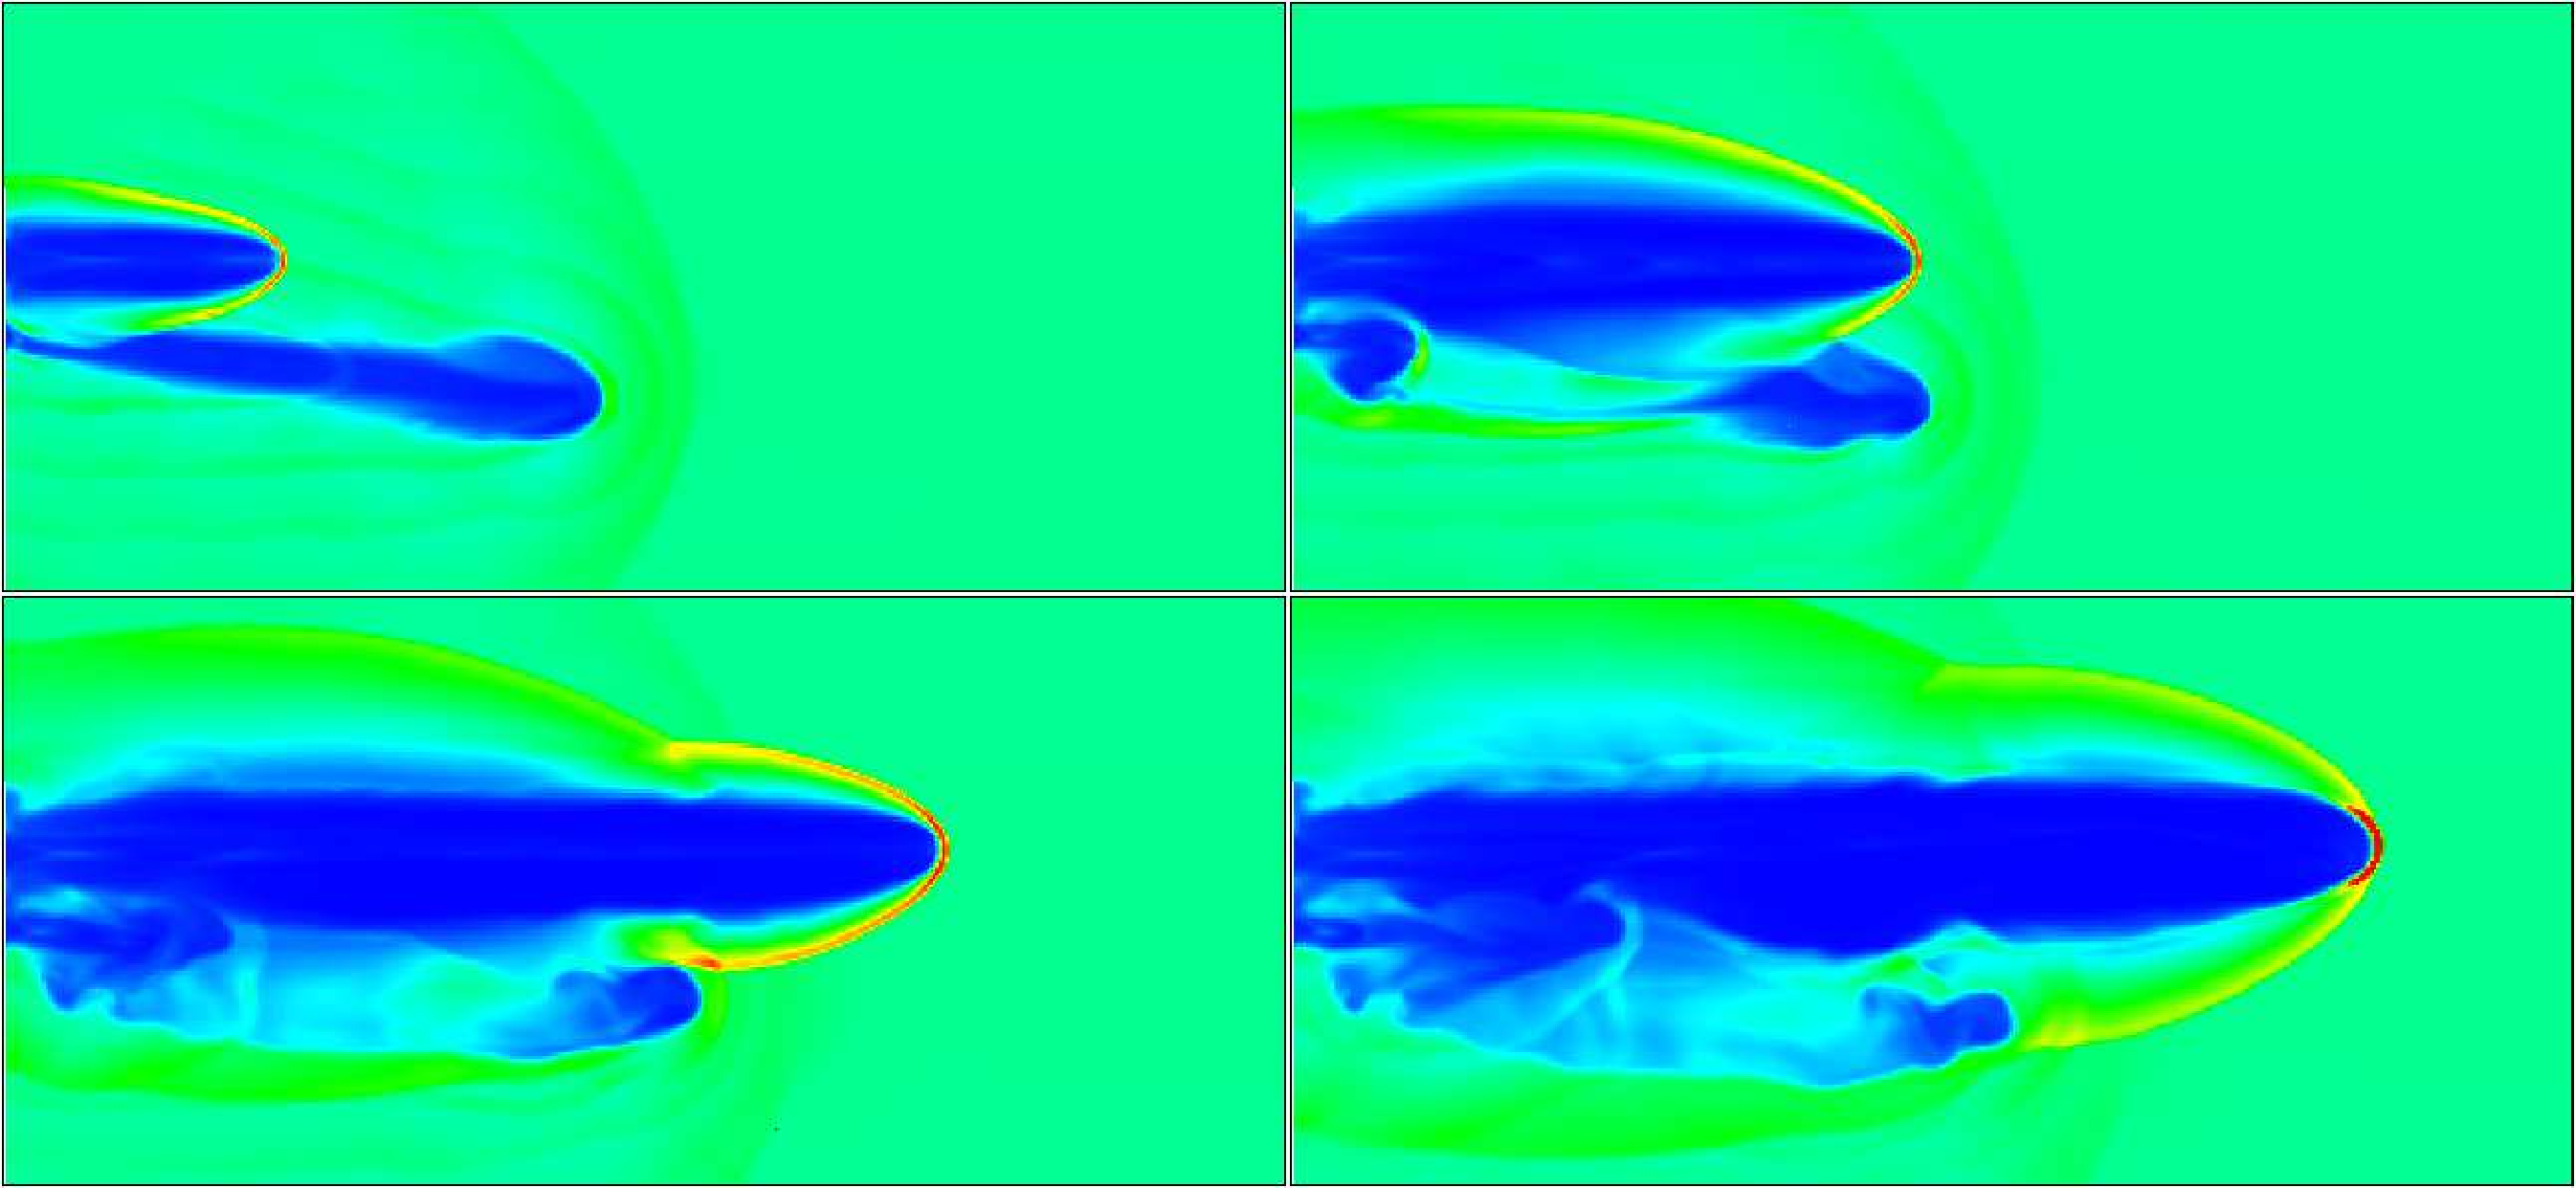
\includegraphics[width=\textwidth]{3d_mhd_twin_jet}
\caption{ 
Time evolution of MHD binary jets at t=125, 155, 170, 185 years. The images shown are
2D midplane cuts through the 3D grid.
Blue is low-density, red is high density.
Note that the angle between jet axes is quite discernable in the earliest panel, but not so much later, which shows the bending of the slow, southern jet over time.
}
\label{fig:4-49}
\end{figure}

Figure \ref{fig:4-49} shows a series of density slices from the 3D MHD
simulation. The binary outflow is modelled in full 3D with a toroidal magnetic field.
%ANALYSIS\\
Compared to the previous HD simulation, where the jets were parallel, the angle between the two jets is initially set to 20$^\circ$. 
As a consequence, one might expect some divergence of the two jets.
On the contrary,
the slower jet is refocused along the faster jet and bends towards it. 
Eventually, the jet material from the slower jet gets merged into the faster one.

% Observations show
The observations  of LDN1551 show both jets diverging from the source 
until about 4$^{\prime\prime}$ from the source when they change 
direction to pursue a roughly parallel course. The change in direction 
is most pronounced for the southern jet.
%which has the lower ram pressure and thus is easier to redirect.
% Simulations show 
In the simulation over the time evolution the southern jet slowly changes its
direction to move parallel to the axis of the toroidal field.
% Physics is
Hence, it appears that the hoop stress from the ambient toroidal field slowly 
changes the direction of the jets.
Thus, magnetised binary jets will tend to collimate and refocus
along the direction of the fastest or strongest jet. 

\subsection{Case III: Orbiting binary jet}

\begin{figure}[t]
\centering
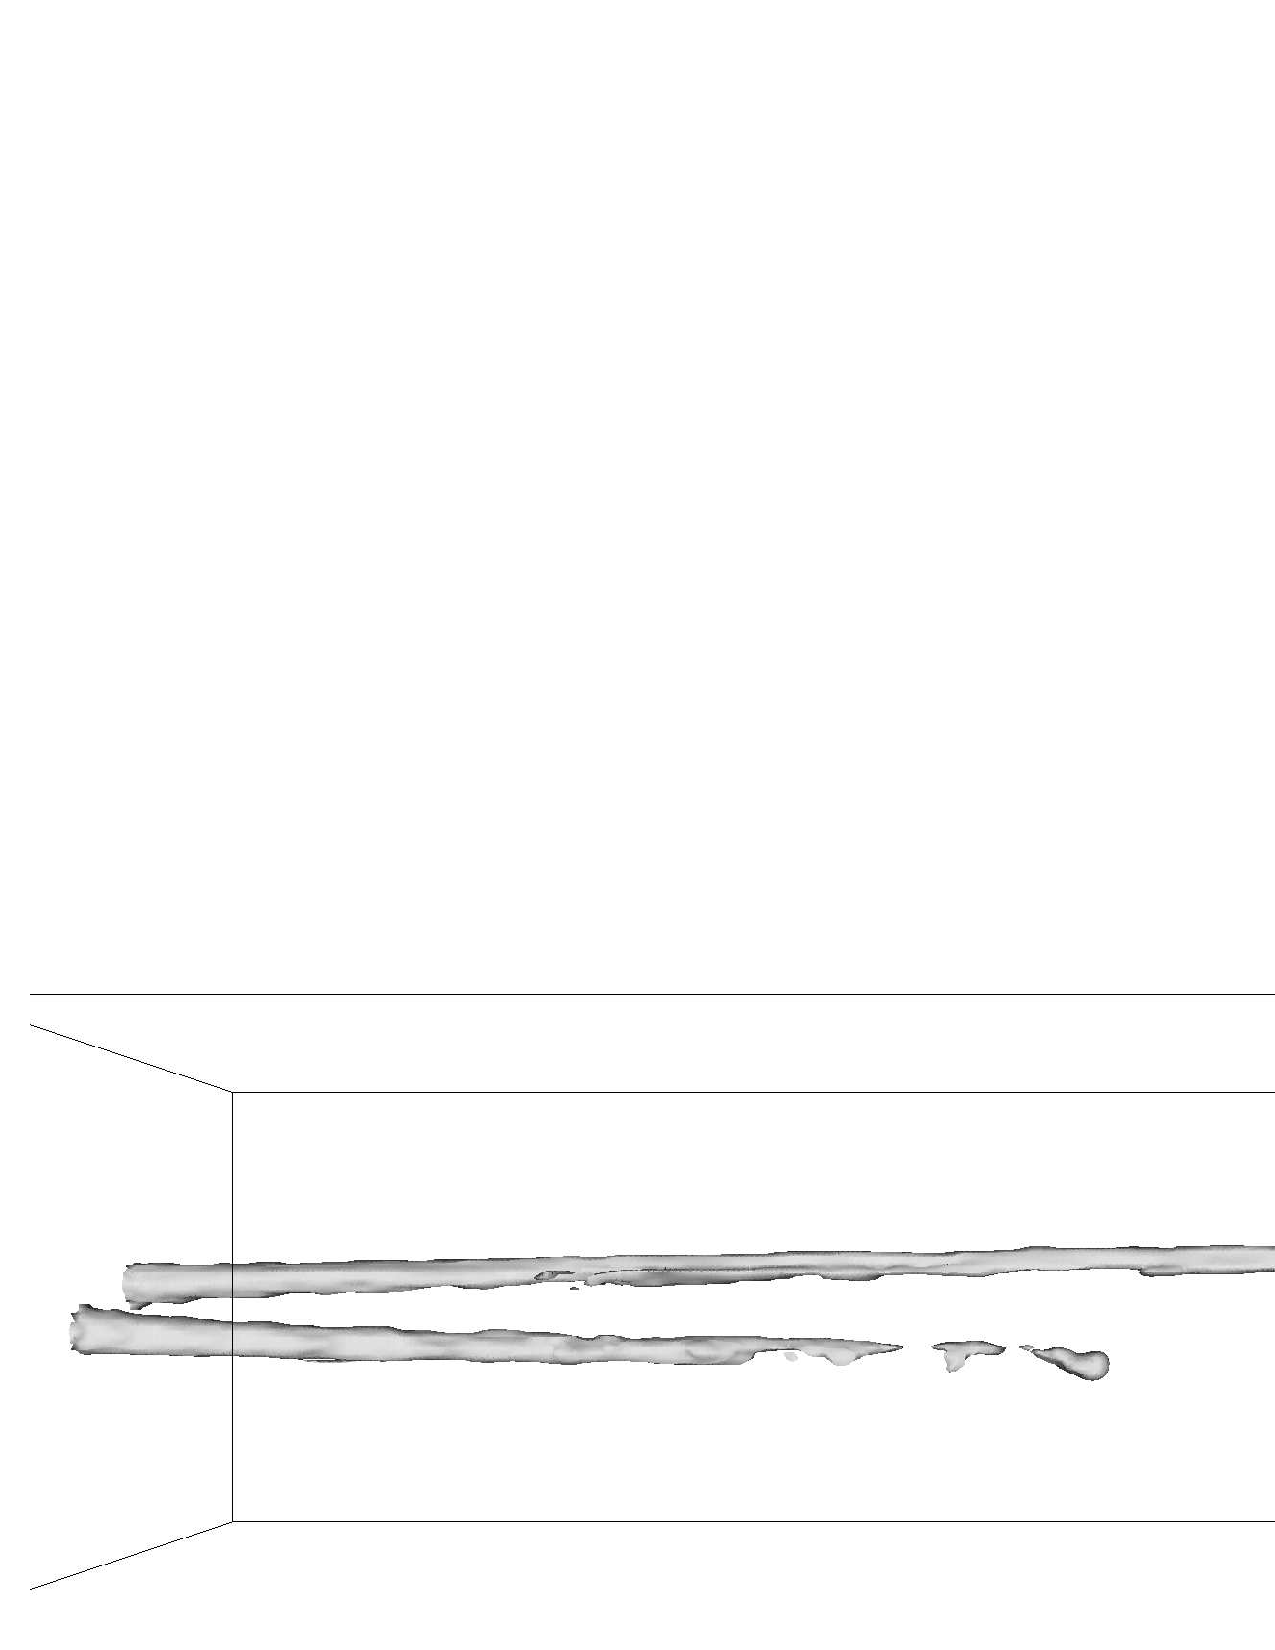
\includegraphics[width=8cm]{3d_surface}
\caption{ 
Surface plot of 3-D binary jet simulation at $t=1648~\mathrm{years}$.
The scale of the grid is $4\times10^{17} \mathrm{cm} \times 10^{17}
 \mathrm{cm} \times 10^{17} \mathrm{cm} $
A longitudinal magnetic field of $10^4 \mu$G is used.
}
\label{fig:4-6}
\end{figure}


The effects of orbital motion on the survival of the binary jets are now explored.
Figure \ref{fig:4-6} shows a model of a binary jet from an orbiting  source. The
model made of two sources consists of one protostar disk orbited by a less massive
companion - both driving jets. The jets have similar velocities and parameters.
It is found that, from time-scale arguments in LDN1551 IRS 5, the orbital period 
of the binary ($\sim$260 years) is too long to have much effect on the fast 
northern jet (dynamical age $\sim$90 years).
The orbit of a binary source may in principle cause the jet to be unstable in
the case of wide binaries with relatively short orbital periods.
Hence, disks orbiting each other are less likely to drive 
coherent visible optical jets, while longer period close binaries 
may drive jets with a visible wiggle e.g. XZ Tau.
Short-period orbits with a large binary separation may cause the binary jet
configuration to be unstable. This is evidently not the case for LDN1551 IRS 5. 
However the binary period represents a powerful constraint on the formation of binary
jets.

\subsection{Emission maps}
%Based on the methods of \citet{2002RMxAC..13....8B} and \citet{2002RMxAC..13...98O} track the ionisation fraction in the medium and post-process the data to produce emission maps.
%The method of \cite{1999A&A...342..717B} is described in that paper and also in \citet{1995A&A...296..185B}. 
%Need to know in advance the temperature, hydrogen nuclear number density, and the fraction of hydrogen ionised. Abundances for the metals are assumed. 
In order to predict the line emission produced by the binary jet model and compare
against observations the density, temperature and the fraction
of ionised hydrogen as computed in the numerical simulations is used. 
Solar abundances for the forbidden line elements in the fluid are assumed.
% Bacciotti code 
Following \citet{2002RMxAC..13....8B}, the emissivity $\epsilon$ is:
\begin{equation}
\epsilon_{Z^i, \nu} = A_{\nu} \frac{hc}{\lambda} x_e n_H^2 
\left( \frac{Z^i}{Z}\right) 
\left( \frac{Z}{H}\right) 
\left( \frac{n_{upper}}{n(Z^i)} \right)
\end{equation}
where
$A_{\nu}$ is the transition probability,
$n_H$ is the hydrogen nuclear number density,
$x_e$ is the ionised fraction of hydrogen.
$ \frac{Z^i}{Z} $ is the fraction of the element Z ionised at level i.
This is set equal to 1 for S, assuming S is all singly ionised in
low-excitation nebula.
For O and N the fractional ionisation may be determined as a function of $x_e$
and $T_e$ assuming the O and N are in ionisation equilibrium with H, and using the
equilibrium rate equations.
$\frac{Z}{H}$ is the abundance of element Z and
$ \frac{n_{upper}}{n(Z^i)}$ is the fractional population of the upper level
- this is determined by a 5-level linear system of equations in $T_e$ and $n_e$.
A more complete description of the method can be found in
\citet{1995A&A...296..185B, 1999A&A...342..717B} and \citet{2002RMxAC..13....8B}.


%\begin{figure}[t]
%\centering
%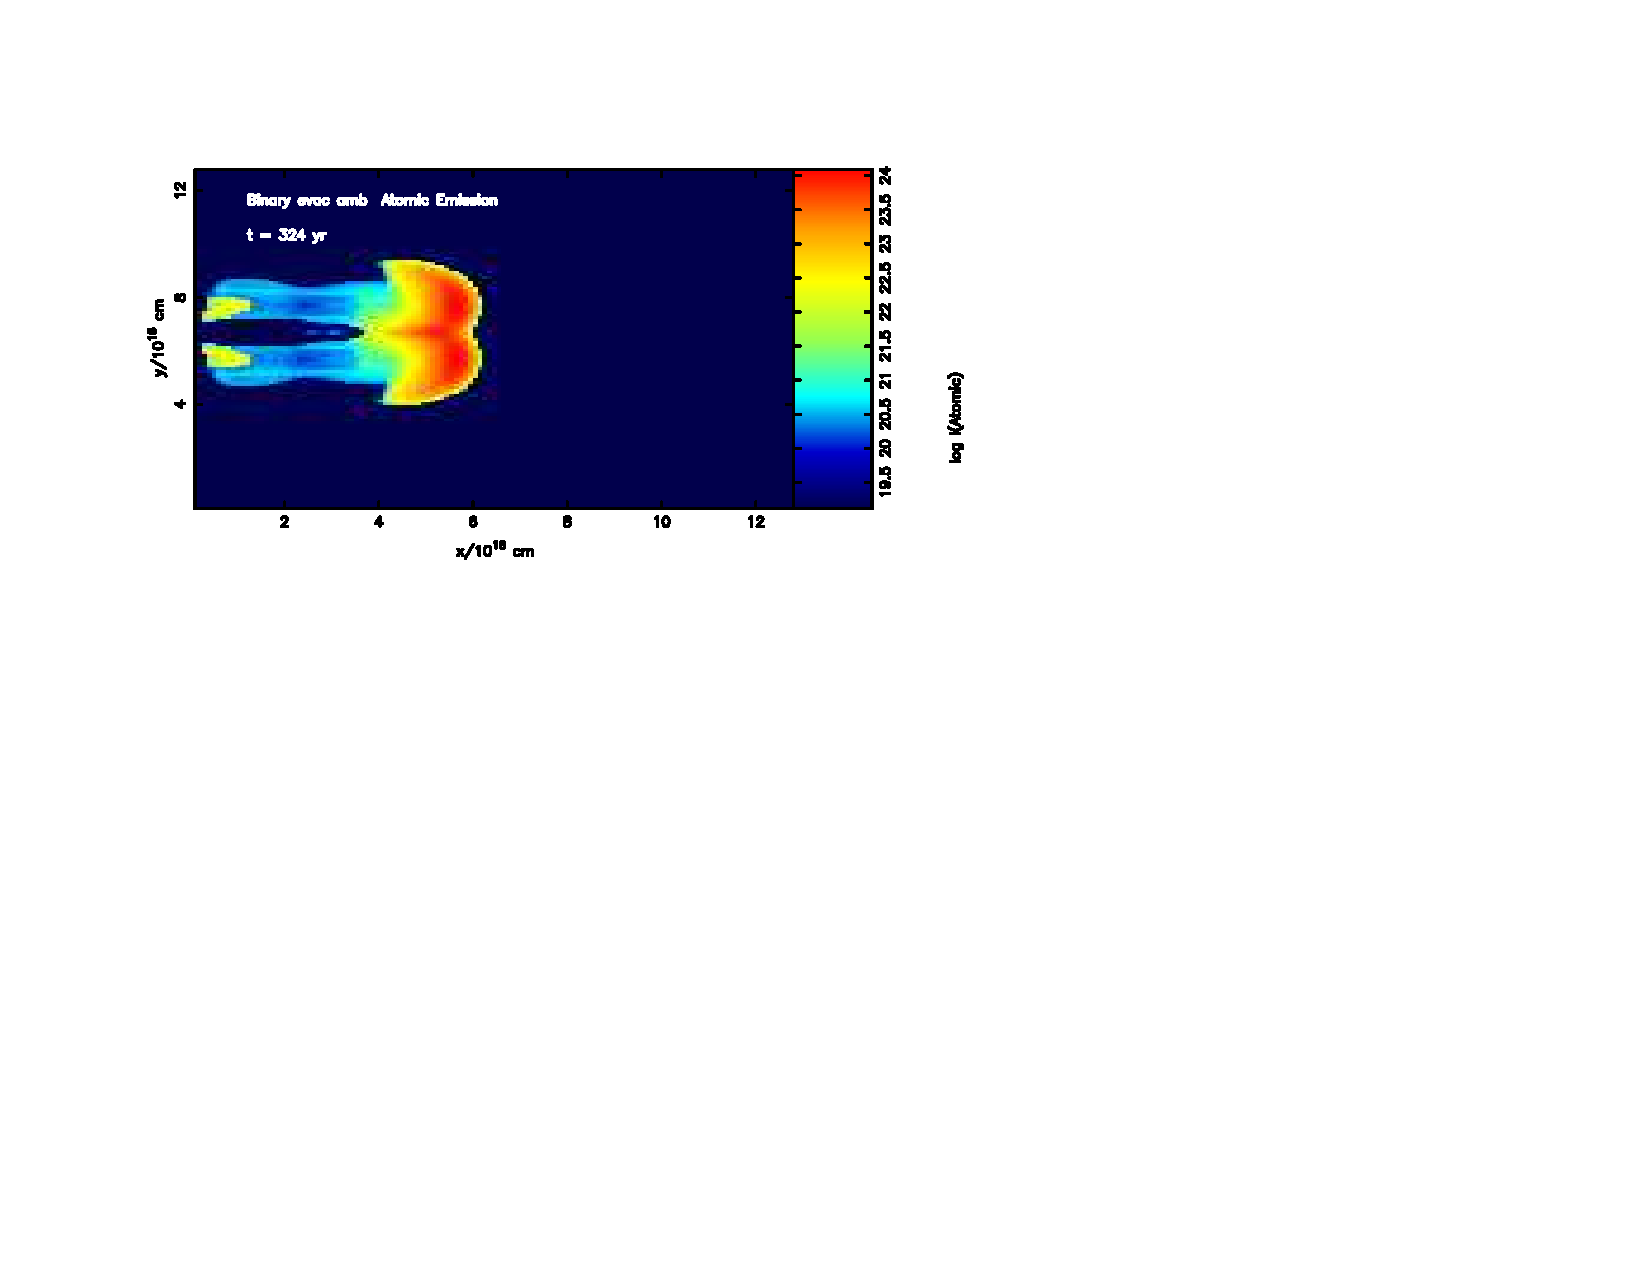
\includegraphics[angle=270,width=8cm]{alex_emission_map}
%\caption{
%Sutherland and Dopita atomic emission map for binary jet system integrated along line-of-sight. This is not the emission from any specific line - but the entirety of instantaneous cooling at the indicated time.
%}
%\label{fig:4-20} 
%\end{figure}



\begin{figure}[t]
\centering
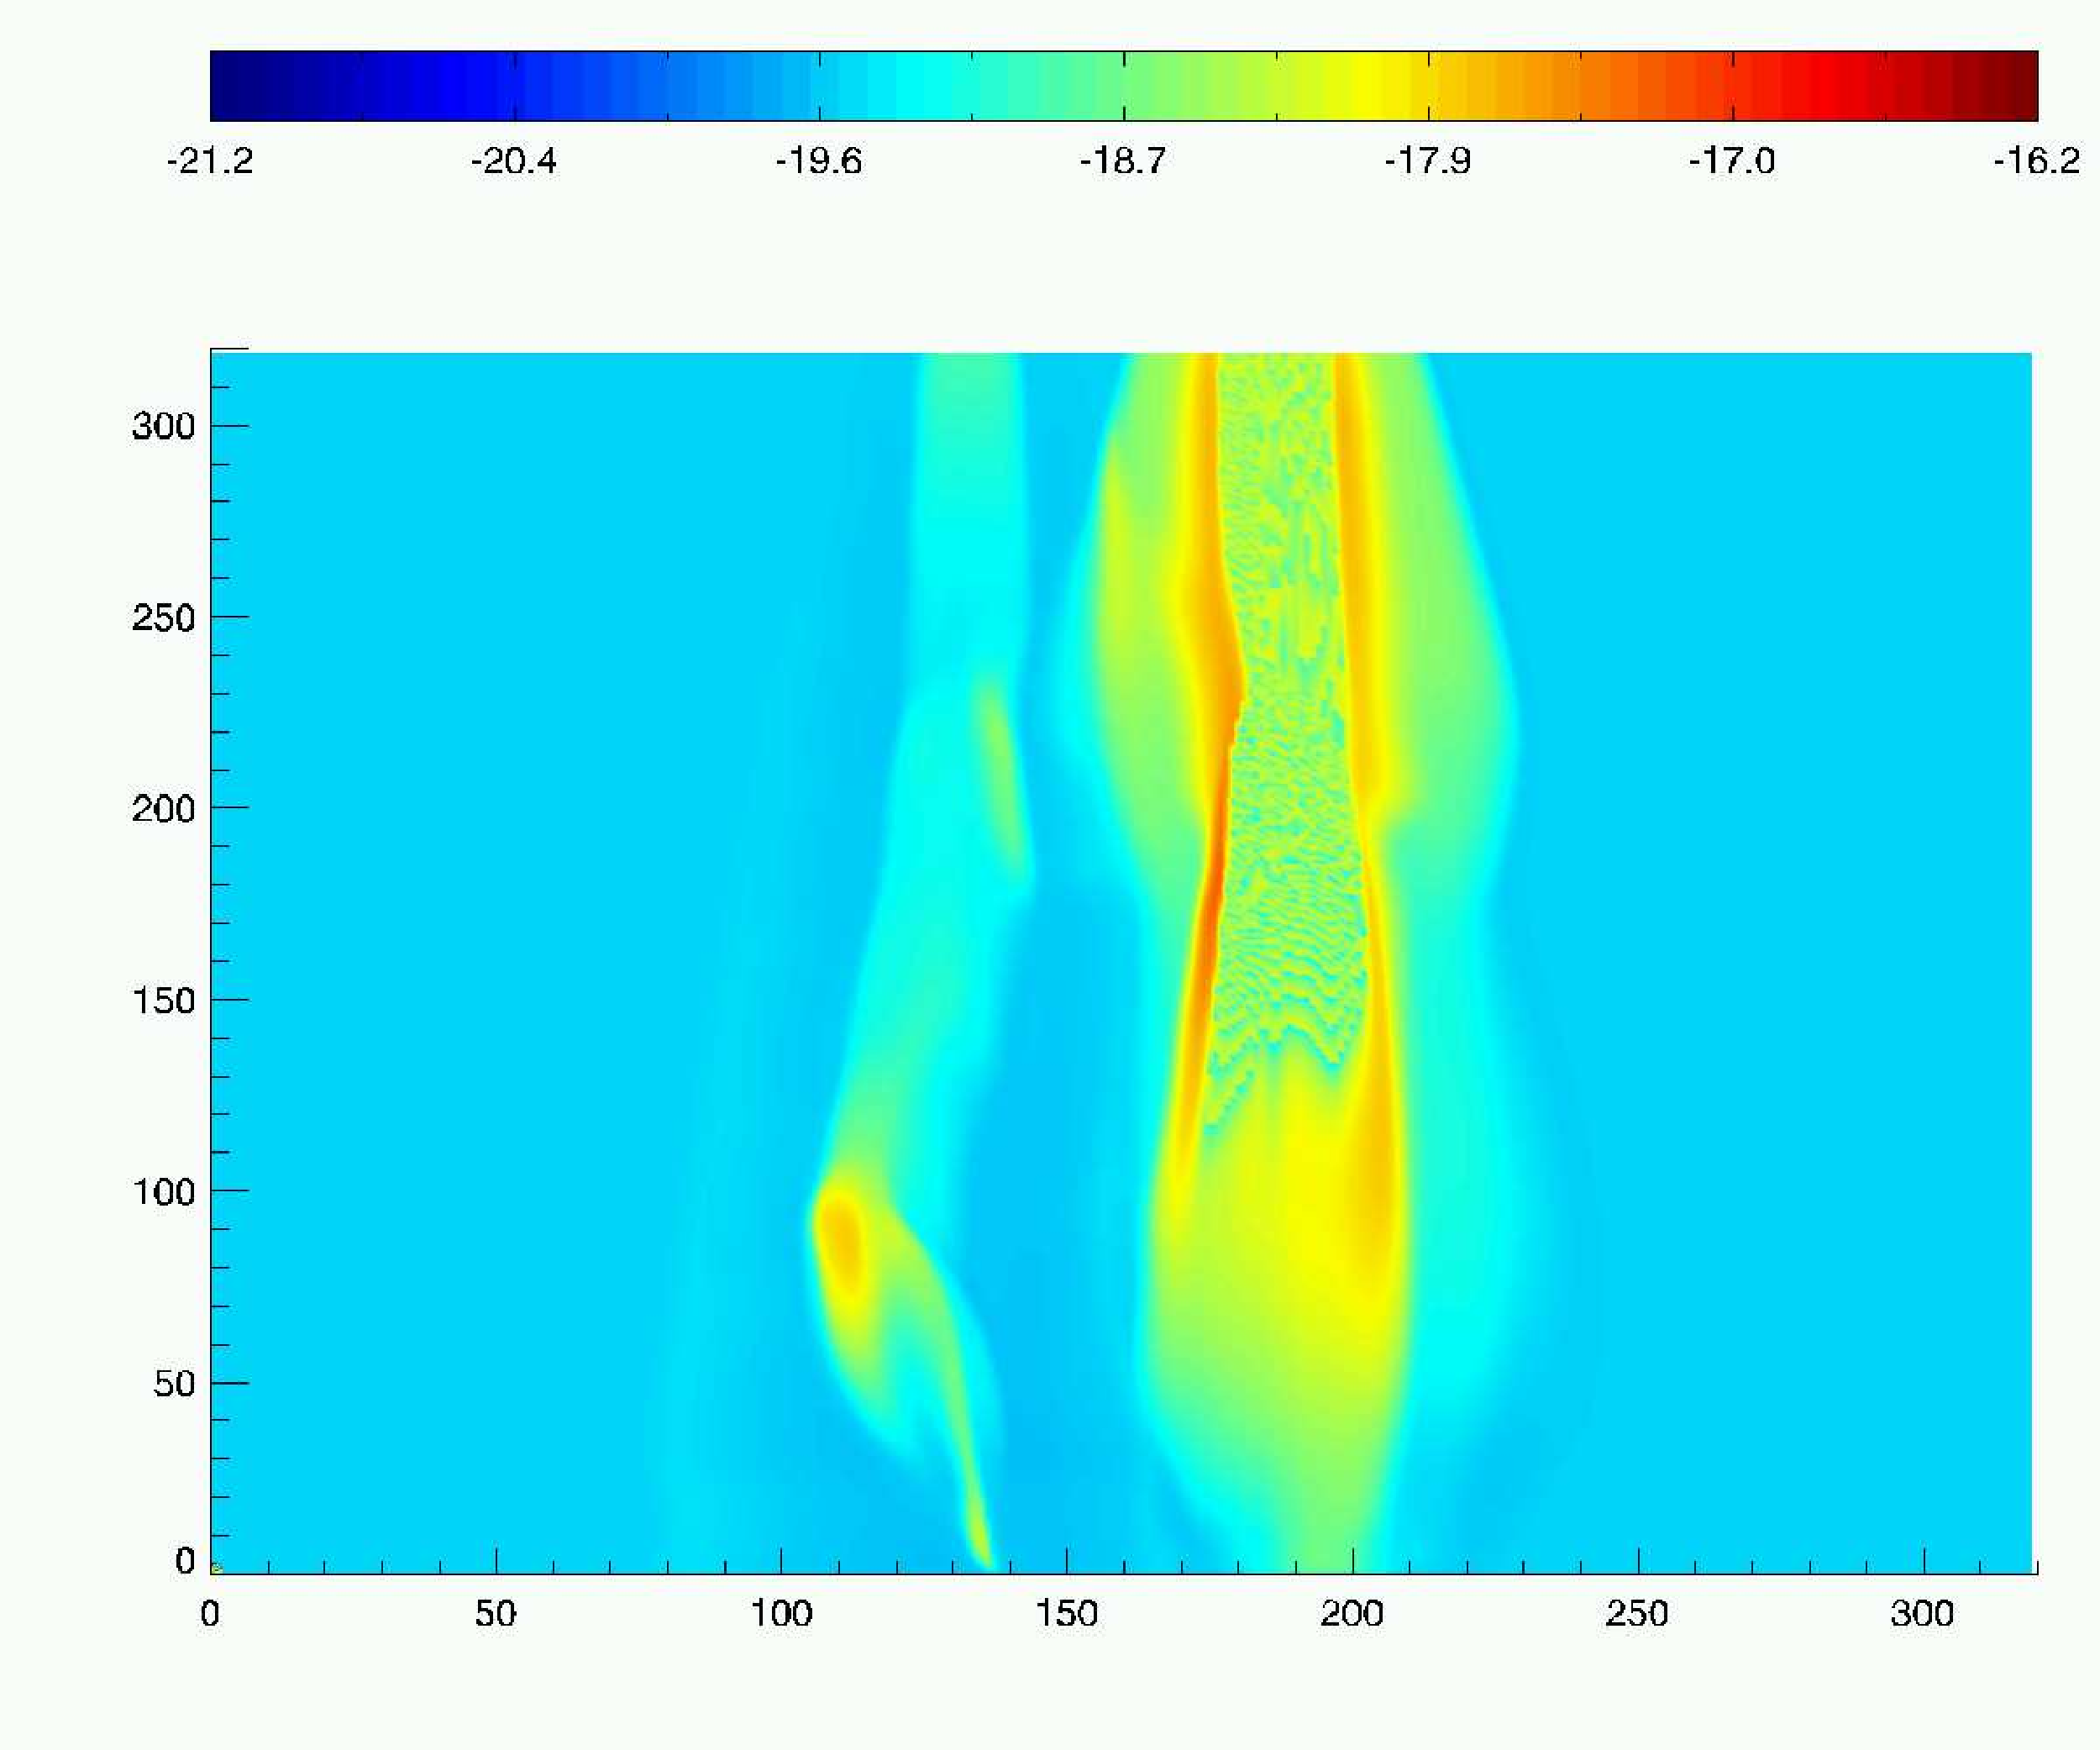
\includegraphics[width=\textwidth]{sii}
\caption{
 [SII] line emission map to compare with observations of the LDN1551 IRS 5 jet (HH154).
 The image shows the lower part of the two jets at a time t=190.2 years.
 The emission map is quite different to what is seen in the density contour and shows that the second jet is almost obliterated by the faster jet. There is a peak in emission where the bow shock is striking the beam.
}
\label{fig:4-21} 
\end{figure}


It is clear from the emission map shown in Figure \ref{fig:4-21} that the interaction has a strong observational signature. The second jet is virtually obliterated but remains visible at the point where the northern jet's bow shock impinges on the beam of the southern jet.



\section{Discussion}\label{Discussion}

\subsection{The source of X-ray emission}
\citet{2003ApJ...584..843B} find a source of X-rays in LDN1551 IRS 5 which they attribute to
either strong shocks \emph{near the base of the jet} or reflected x-rays scattered out through the outflow cavity.
The strong shocks may be caused by jet collimation which could be magnetic in nature. 
\citet{2004A&A...424L...1B} correctly predicted the proper motion of the X-ray source.
In the binary jet model the X-ray source could possibly come from the colliding winds as
suggested in \citet{2003ApJ...584..843B}.
The Bally model suggests that the X-rays come from a moving source at the base
of the jets. If the density ratio is $n_{jet}/n_{ambient}=0.1$ then the shock speed
will be about 430/4=107 too slow to achieve X-ray emission temperatures. If on
the other hand the density ratio is higher (e.g. 10) the jet is moving into a less
dense region swept out by the slower jet the shock velocities will be higher
430*0.75 = 322. To get up to the observed shock velocity the density contrast would
need to be much lower than observed e.g. 0.01 would give a velocity in the range required.
The X-ray emission may then be more likely to originate in the binary source.
Another possibility is that the X-ray emission is caused by magnetic reconnection in the
interval between the two jets where the field is compressed by the pair of bow
shocks. 

% Implications for jet launching
%(Any binary jet would have significant implications for the role of magnetic fields in jet launching.)

\subsection{Magnetic field effects}
Magnetic field direction has a strong effect on the direction and magnitude of jets.
\citet{1986ApJS...62...39S} and \citet{1989AJ.....98.1368T} showed magnetic fields near young stars appears to be preferentially aligned with jet axes, where jets exist. 
On the other hand \citet{2004A&A...425..973M} have 
suggested that magnetic fields are orientated randomly.
In the case of LDN1551 IRS 5, the observations of the perpendicular magnetic
field projected in the plane of the sky imply a toroidal field in the ambient medium surrounding the jet. 
The results from Section \ref{sec:BinJetMHD} show that such a toroidal field would affect the motion of the southern jet; and
that both the magnetically driven change in direction together with the interaction
of the bow shock of the fast jet with the beam of the slow jet contribute to the
distinctive morphology.

\subsection{Source orbiting effects}
An orbiting source can cause jet precession.
Indeed, \citet{2002ApJ...568..733M} have used this effect to explain the wiggling of the jet associated with HH30.
However in the particular case of LDN 1551 IRS 5, the period of oscillation is too long to have a very significant
effect on either of the two jets over the length scale and timescale of interest here. 
However the LDN 1551 IRS 5 jets drive a massive ($\sim$0.5 parsec ) molecular outflow, and the stirring motion produced by the 300 km~s$^{-1}$ two jets orbiting the source may contribute to the morphology of the 15 km~s$^{-1}$ molecular outflow.
Decreasing the orbital period contributes to the jet
breaking up -- as the jet orbits it has to do extra work moving the ambient medium in a lateral direction.
This has the effect of a transverse wind, shredding the jet.
Obviously this is effect is small enough for the observed jets so they may be observed.
However a short period binary should not be able to produce a
stable jet especially if it is a wide binary. This is a major constraint on the
production of binary jets.

\subsection{Jet merging}

In the case of LDN1551 IRS 5 the two jets appear to merge into a single bow shock
at about 1400 AU from the source. However this effect is only apparent and
although the jets appear to be bent either by the local variations in the
density or the surrounding toroidal field they do not merge into a single jet.

The LDN1551 IRS 5 jet pair can be seen as both a pathological object unlike any other observed at such close range and as an ideal candidate for attempted explanation of the observed phenomena using a hydrodynamical code. The effects of source orbiting, density parameters, magnetic fields all play a role in sculpting this most unusual object which is the nearest protostellar jet visible in the optical.



\section{Conclusions}

From the three-dimensional numerical simulations of interacting binary jets, several results are apparent.
\begin{itemize}
\item 
For the underdense jets in this simulation, when the jets interfere, 
either they survive as two jets if the sources have a large spatial or angular separation, 
or merge into one single jet if the sources have a small spatial separation. 
Dense ballistic jets are however much less likely to interact than light jets.

%Bending of the jets in LDN1551
\item Using the observed parameters as far as possible, the kink and projected bending of the secondary jet has been reproduced as observed for LDN1551 IRS 5.

%Orbital effects
\item Over a long time-scale, precession induced by the orbital motion of the source is seen.
On the short lifetime of the jets from LDN1551, this effect is negligible. 

% MHD effects
\item If the jets are not strictly parallel, as in most of the limited set of observed binary protostellar jets, it is shown that
the toroidal magnetic field like the one simulated here, in the ambient medium though which the jets propagate, can help the collimation and refocusing of both the jets.

%Emission maps
\item In the comparison of the emission maps against the observations
it is shown that the kink structure of interacting jets is still apparent in the synthetic 
observations. 
%with a strong emission at the head of the jets.

%Binary vs single jets

\end{itemize}

